% \chapter{Makefile Examples}
\label{part:examples}

\begin{vplace}[0.7]
	
	\thispagestyle{empty}
	\large
	\noindent This part includes examples of Makefiles included in the practical data. We assume that you have unzipped the practical data into a directory somewhere in your local environment. Once you have done that, you should set an environment variable called \texttt{MAKEPIPELINES} to refer to this directory. In the command below we assume you have placed it in your home directory:
	\bashcmd{export MAKEPIPELINES=\textasciitilde{}/makepipelines}
	
	The examples included below will reference this environment
        variable as necessary to find the correct files.

        Please contact the example's author with questions,
        or Katie Askren or Tara Madhyastha where no specific author is listed.
	
\end{vplace}

\newgeometry{scale=0.85, centering}
\definecolor{lemon}{HTML}{F5ECCE}

\lstset{language=make,backgroundcolor=\color{lemon},showstringspaces=false,
	gobble=8,
	basicstyle=\small\ttfamily,
	breaklines=true,
	escapeinside={\%*}{*}}
 % this is in the same directory

% % IN ALL CHAPTER HEADINGS USE \Echapter{title}{author}

%% Do not use underscores in input file names - 
\setcounter{codehighlight}{0}
\Echapter{Downloading Data From XNAT}{Karl Woelfer}{kwoelfer@uw.edu}
\label{chap:XNAT}

This is an example of how to use a Makefile to create and populate a
project directory with images from an open dataset stored in an XNAT
(eXtensible Neuroimaging Archive Toolkit) database, in this case from
the NITRC (Neuroimaging Informatics Tools and Resources Clearinghouse)
1000 Functional Connectomes project image repository at
\url{http://www.nitrc.org/ir}. The code for this example is located at \texttt{fcon_1000/Makefile}.

To run this pipeline you will need to have first created an individual
user account on NITRC, at
\url{http://www.nitrc.org/account/register.php}, and obtained access
to the 1000 Functional Connectome project.

To simplify this example, we download only a subset of the subjects in
the repository. A file with the names of these subjects is used to
determine what files to download.

In our example, we selected 23 Baltimore subjects, saved in the file \texttt{Subjects_Baltimore}.
To recreate this file you can do the following. From the NITRC Image Repository home page ``Search,'' choose Projects $\rightarrow$ 1000 Functional Connectomes. At the 1000 Functional Connectomes project home page, select Options $\rightarrow$ Spreadsheet to download a CSV file of the 1288 subjects \texttt{AnnArbor_sub00306 \ldots Taipei_sub91183}. Select a subset, or all, of the subjects from the first column of the downloaded spreadsheet, and save to a text file. 

The directory hierarchy that this Makefile creates under your project home, from which \maken{} is run, is shown in \autoref{fig:xnat-dir}. Note
that this Makefile assumes that the directory \texttt{visit1} already exists.

\begin{figure}
	\dirtree{%
		.1 fcon_1000/.
		.2 subjects/.
		.3 Baltimore_sub17017/.
		.4 visit1/.
		.5 rest.nii.gz.
		.5 T1_brain.nii.gz.
		.5 T1.nii.gz.
		.3 Baltimore_sub19738/.
		.4 visit1/.
		.5 rest.nii.gz.
		.5 T1_brain.nii.gz.
		.5 T1.nii.gz.
		.3 \ldots.
		.2 visit1/.
		.3 Baltimore_sub17017/\DTcomment{A symlink to ../subjects/Baltimore_sub17017/visit1}.
		.3 Baltimore_sub19738/.
		.3 \ldots.
	}
		\caption{XNAT access directory structure.}
			\label{fig:xnat-dir}
\end{figure}


\begin{lstlisting}
	# Site hosting XNAT
	%*\lnote*NITRC=http://www.nitrc.org/ir
	
	%*\lnote*SHELL=/bin/bash
	
	# Obtain the list of subjects to retrieve from NITRC
	%*\lnote*SUBJECTS = $(shell cat Subjects_Baltimore)

	%*\lnote*.PHONY: clean all allT1 allT1_brain allrest allsymlinks
\end{lstlisting}

This portion of the Makefile defines key variables and targets. 

\indent \lnum{1}We set the ``base name'' of the XNAT web site in a variable \texttt{NITRC}. This can be changed when using another XNAT repository, and the variable can be named accordingly. \\
\indent \lnum{2} By default, \maken{} uses \texttt{/bin/sh} to interpret recipes. Sometimes this can cause confusion, because \texttt{sh} has only a subset of the functionality of \texttt{bash}. We set the \maken{} variable \texttt{SHELL} explicitly. \\
\indent \lnum{3}The \texttt{SUBJECTS} variable will contain a list of the subject data we wish to download. The individual subject names will be used to create directory names. \\
\indent \lnum{4}We define six targets that do not correspond to files, so these are denoted as phony targets.

\begin{lstlisting}
	%*\lnote*all: sessionid allT1 allT1_brain allrest allsymlinks
	%*\lnote*allT1: $(SUBJECTS:%=subjects/%/visit1/T1.nii.gz)
	%*\lnote*allT1_brain: $(SUBJECTS:%=subjects/%/visit1/T1_brain.nii.gz)
	%*\lnote*allrest: $(SUBJECTS:%=subjects/%/visit1/rest.nii.gz)
	%*\lnote*allsymlinks: $(SUBJECTS:%=visit1/%)
\end{lstlisting}

\indent \lnum{5} \texttt{all} is the default target, and simply defines the five dependencies. \\
\indent \lnum{6} We need to derive the names of all the files that we
intend to create from the list of subjects. We do this using pattern
substitution to define several targets. Here, we use pattern matching
to generate a list of the T1 image names that we need to create. Each of
the subject names, e.g. \texttt{Baltimore_sub17017}, is used to create
the corresponding T1 image (e.g. \texttt{subjects/Baltimore_sub17017/visit1/T1.nii.gz}).\\
\indent \lnum{7} As above, we form the names of the skull stripped T1 images.\\
\indent \lnum{8} And the resting state images.\\
\indent \lnum{9} The last thing the Makefile does is create a
\texttt{visit1/} directory after the \texttt{subjects/} directory has
been populated. Here we use pattern matching, as above, to generate
the list of symbolic links that need to be created.  Each
\texttt{visit1/SUBJECT} directory will be a symbolic link to the actual \texttt{subjects/SUBJECTS/visit1/} directory.


\begin{lstlisting}
	%*\lnote*sessionid: 
		@echo -n "Username: " ;\
		read username ;\
		curl --user $$username $(NITRC)/REST/JSESSION > $@
\end{lstlisting}

\indent \lnum{10} Here we use the client URL Request Library
(\texttt{cURL}) to create a session with the XNAT server. The first
line prompts for the user's name on the XNAT server, the second line
reads and stores that in the variable \texttt{username}. With one
single REST transaction, the \texttt{cURL} call on the following line,
we authenticate with the XNAT server, entering a password only once,
and saving the return value \texttt{SESSIONID} in a file named
\texttt{sessionid}. This single session will persist for an
hour. Obtaining a session identifier is important to reduce load on
the remote XNAT server.
	
\begin{lstlisting}	
	%*\lnote*subjects/%/visit1/T1.nii.gz:  | sessionid
	%*\lnote*	mkdir -p `dirname $@`; \
	%*\lnote*	curl --cookie JSESSIONID=`cat sessionid` $(NITRC)/data/projects/fcon_1000/subjects/$*/experiments/$*/scans/ALL/resources/NIfTI/files/scan_mprage_anonymized.nii.gz > $@

\end{lstlisting}

\indent \lnum{11} This recipe downloads all of the T1 images required
by target \texttt{allT1} (\lnum{6}). It has an order-only dependency
upon the file \texttt{sessionid} because we assume that if these files
exist, it does not matter if they are older than the
\texttt{sessionid} file. They will only be recreated if they do not
exist. \\
\indent \lnum{12} This command creates the directory
\texttt{subjects/SUBJECT/visit1} if it does not exist (where SUBJECT
is the actual subject identifier).\\
\indent \lnum{13} This \texttt{curl} command uses the
\texttt{SESSIONID} which was stored in the \texttt{sessionid}
file. The URL defined here is specific to the location where scan data
of interest is stored on the NITRC instance of XNAT. Note that
\texttt{\$*} is used in two places to refer to the subject identifer, denoted by
\texttt{\%} in the target. The XNAT file \texttt{scan_mprage_anonymized.nii.gz} is downloaded and saved under the local name \texttt{T1.nii.gz}.

\begin{lstlisting}
	$subjects/%/visit1/T1_brain.nii.gz:  | sessionid
		mkdir -p `dirname $@`; \
		curl --cookie JSESSIONID=`cat sessionid` (NITRC)/data/projects/fcon_1000/subjects/$*/experiments/$*/scans/ALL/resources/NIfTI/files/scan_mprage_skullstripped.nii.gz > $@
\end{lstlisting}

\indent This recipe is analogous to the previous one, except
that it creates the skull stripped T1 images needed by target
\texttt{allT1_brain}.

\begin{lstlisting}
	subjects/%/visit1/rest.nii.gz:  | sessionid
		mkdir -p `dirname $@`; \
		curl --cookie JSESSIONID=`cat sessionid` $(NITRC)/data/projects/fcon_1000/subjects/$*/experiments/$*/scans/ALL/resources/NIfTI/files/scan_rest.nii.gz > $@
\end{lstlisting}

\indent Similarly, this recipe creates the resting state
images needed by \texttt{allrest}.


\begin{lstlisting}
	visit1/%:
		ln -s ../subjects/$*/visit1 $@
\end{lstlisting}

\indent  This recipe populates the project top-level \texttt{visit1/} directory with symbolic links, pointers to the actual locations of the subjects' \texttt{visit1} data downloaded above. This enables an alternate way to access the subject data.

\begin{lstlisting}
	clean:
		rm -rf subjects; \
		rm -rf visit1/*; \
		rm -f sessionid
\end{lstlisting}

This \texttt{clean} recipe will delete everything in
\texttt{subjects/}, links in the \texttt{visit1/} directory, and the
\texttt{sessionid} file.

 \clearpage \setcounter{codehighlight}{0}
\chapter{Running FreeSurfer}
\def\sectionautorefname{Running Freesurfer}
\label{chap:freesurfer}

This is an example of how to use a makefile to execute FreeSurfer's longitudinal pipeline. Note that FreeSurfer itself is a large pipeline built using \texttt{make}. However, we do not need to know that if we treat the program \texttt{recon-all} as a single executable and show how to use \maken{} to call it. Here, the Makefile functions more as a way to permit parallel execution of \texttt{recon-all} rather than a way to track dependencies. 

The code for this example is in \texttt{oasis-longitudinal-example-small/freesurfer/Makefile}.

\setcounter{codehighlight}{0} % RESET THIS BEFORE EVERY LST LISTING
\begin{lstlisting}
	PROJHOME=$$MAKEPIPELINES/oasis-longitudinal-sample-small
	%*\lnote*SUBJECTS_DIR=$(PROJHOME)/freesurfer

	QA_TOOLS=/usr/local/freesurfer/QAtools_v1.1
	FREESURFER_SETUP = /usr/local/freesurfer/stable5_3/SetUpFreeSurfer.sh
	RECON_ALL = /usr/local/freesurfer/stable5_3/bin/recon-all $(RECON_FLAGS)	
	%*\lnote*RECON_FLAGS = -use-mritotal -nuintensitycor-3T -qcache -all  -notal-check

	%*\lnote*SHELL=/bin/bash
\end{lstlisting}

\lnum{1}FreeSurfer normally likes to work with all subjects in a single directory. We set the \maken{} variable \texttt{PROJHOME} for convenience, and the \texttt{SUBJECTS_DIR} because it is required by FreeSurfer. \\
\indent\lnum{2}Because we have multiple versions of FreeSurfer installed, and because it is possible to run FreeSurfer with different flags, we set several variables that describe what version of FreeSurfer and what options we are using in the Makefile. Note that the definition for \texttt{RECON_ALL} refers to \texttt{RECON_FLAGS} seemingly before it is set. Recall that \maken{} dereferences variables when it uses them, so the order that these variables are set does not matter. This is not like \texttt{bash}!\\
\indent\lnum{3}By default, \maken{} uses \texttt{/bin/sh} to interpret recipes. Sometimes this can cause confusion, because \texttt{sh} has only a subset of the functionality of \texttt{bash}. We can avoid such confusion by setting the \maken{} variable \texttt{SHELL} explicitly.


\begin{lstlisting}
	%*\lnote*SUBJECTS=$(notdir $(wildcard $(PROJHOME)/subjects/*))	
\end{lstlisting}

\lnum{4}We need to obtain a list of subject identifiers to process. Here, we form this list by using a wildcard to obtain all the subject directories in \texttt{PROJHOME} and then stripping away all the directory prefixes using the \texttt{notdir} call.


\begin{lstlisting}
	SESSION=1
	%*\lnote*inputdirs=$(SUBJECTS:%=%.t$(SESSION))

	%*\lnote*.PHONY: qa setup freesurfer

	%*\lnote*setup: $(inputdirs)

	%*\lnote*%.t$(SESSION):  $(PROJHOME)/subjects/%/visit$(SESSION)/mpr-1.nifti.nii.gz
            mkdir -p $@/mri/orig; \
        	cp $^ $@/mri/orig; \
        	cd $@/mri/orig; \
        	mri_convert mpr-1.nifti.nii.gz 001.mgz
\end{lstlisting}

\lnum{5}This Makefile is intended to handle a longitudinal acquisition. Normally, one indicates the timepoint (here, the \texttt{SESSION} variable indicates the timepoint) by appending some suffix to the subject identifier. Here, we append the suffix \texttt{.t1} to each subject identifier to indicate that we are processing the first session. To run the makefile on the second timepoint, one could either edit it, or set this variable when calling \maken{} as follows:
\bashcmd{make SESSION=2}

\indent\lnum{6}We define three targets that do not correspond to files, so these are denoted as phony targets.\\
\indent\lnum{7}The phony target \texttt{setup} depends upon the input directories we defined in \lnum{6}.\\
\indent\lnum{8}This recipe creates the input directories by transforming the first MPRAGE image from the subject directory into mgz format. More complicated recipes may include conditionally choosing one of multiple MPRAGE images, using two images if available, and so forth. 


\begin{lstlisting}
	freesurfer: $(inputdirs:%=%/mri/aparc+aseg.mgz)

	%*\lnote*%.t$(SESSION)/mri/aparc+aseg.mgz: $(PROJHOME)/subjects/%/visit$(SESSION)/mpr-1.nifti.nii.gz
        	rm -rf `dirname $@`/IsRunning.*
	        source $(FREESURFER_SETUP) ;\
        	export SUBJECTS_DIR=$(SUBJECTS_DIR) ;\
        	$(RECON_ALL) -subjid $*.t$(SESSION) -all
\end{lstlisting}

\lnum{9} FreeSurfer creates many output files when it runs. Here, we select one of the critical files that should exist upon successful completion, \texttt{mri/aparc+aseg.mgz} to be the target of this rule. It depends upon the directory having been created so that we can call \texttt{recon-all} by specifying the subject directory. You might think that it would be wise to specify multiple FreeSurfer output files as targets. In this case, if the multiple targets are specified using a pattern rule, the recipe would be executed only once to create the targets. However, if we did not use a pattern rule, the recipe could be executed once per target. This is clearly not the intended behavior. To avoid confusion, we usually pick a single late-stage output file to be the target.


\begin{lstlisting}
	%*\lnote*qa: $(inputdirs:%=QA/%)

	%*\lnote*QA/%: %
        	source $(FREESURFER_SETUP) ;\
        	$(QA_TOOLS)/recon_checker -s $*
\end{lstlisting}

\lnum{10}We can create a number of quality assurance (QA) images from the FreeSurfer directories using the \texttt{recon_checker} program. The \texttt{qa} target depends upon directories within the \texttt{QA} subdirectory. These are created by \texttt{recon_checker} in \lnum{12}.


\begin{lstlisting}
	%*\lnote*Makefile.longitudinal:
		$(PROJHOME)/bin/genctlongitudinalmakefile > $@
\end{lstlisting}

\lnum{11}After all the cross-sectional runs have been completed, we can run the longitudinal pipeline. The first step in this pipeline is to create an unbiased template from all timepoints for each subject. The second step is to longitudinally process each timepoint with respect to the template.

Here, we have a bit of a problem specifying these commands to \maken{} because each subject may have a different number of timepoints and subjects may be missing a timepoint that is not the first or last. The syntax of the \texttt{recon-all} command to create an unbiased template does not lend itself well to using wildcards to resolve these issues:
\bashcmd{recon-all -base <templateid> -tp <tp1id> -tp <tp2id> ... -all}

We solve these problems by writing a shell script that generates a correct Makefile (\texttt{Makefile.longitudinal}). This is an example of taking a ``brute force'' approach rather than trying to use pattern rules or something more sophisticated. It gets the job done.

The new makefile defines a target \texttt{longitudinal}, and can be called as follows, adding additional flags for parallelism.
\bashcmd{make -f Makefile.longitudinal longitudinal}
 \clearpage  \setcounter{codehighlight}{0}
\Echapter{DTI Distortion Correction with Conditionals}{Daniel J. Peterson}{djpeters@uw.edu}
\label{chap:dti}

In this example, we will use a Makefile to apply the appropriate
distortion correction procedure automatically, using conditionals. The
code for this example may be found in
\texttt{dti_suceptibility_correction/subjects}, in Makefiles in the
directories \texttt{fugue_DTI}, \texttt{topup_DTI}, and
\texttt{toy_test} as described below.

First, a bit of background: The most common way to acquire a series of
MRI images as quickly as possible is to use what is called an
``echo-planar imaging readout,'' or ``EPI.'' A drawback that comes
with this rapid acquisition is that EPI images are prone to
distortions due to an uneven magnetic field. Sometimes these
distortions are called ``susceptibility-induced distortions,'' because
it is the differing magnetic susceptibility of tissue, bone, and air
that causes the magnetic field to be uneven. Fortunately, because these
distortions are constant and predictable within an imaging session,
they can be undone.

We will consider two ways of undoing these distortions, each requiring
at least one extra image to be acquired. The first method is to
acquire an image of the uneven magnetic field, called a ``fieldmap.''
This image contains a map of the deviation from the main magnetic
field, in radians/sec (the resonance frequency of the water protons is
directly proportional to the strength of the magnetic field as per the
Larmor equation: $\omega=\gamma B _{0}$). To do this we will use a
tool called \texttt{fugue}, which is distributed as part of
FSL. \texttt{fugue} will convert this fieldmap into a nonlinear warp,
and then we can apply that warp to undo the susceptibility-induced
distortions. The other method is to acquire an additional image with
the EPI readout going in the other direction, meaning that the
direction of the susceptibility-induced distortion will be
reversed. We can then use a tool called \texttt{topup} (also from
FSL), that will warp two images with opposite distortions towards each
other, until they meet in the middle. We can then apply this computed
warp to the rest of our data.


These are two different procedures that require different sets of
files (an acquisition parameters file for \texttt{topup} and a
fieldmap for \texttt{fugue}), but can be part of an otherwise similar
pipeline. We can use \maken{} to sense which procedure to use based on
what files are present, and assemble the appropriate prerequisites.


To help understand the behavior of \maken{}, we have created an
example of a ``toy'' makefile, which does not call any real programs,
and can operate on empty ``dummy'' files. When debugging and
developing makefiles it can be useful to write such simplified
makefiles, and run them with \maken{}~\texttt{-n}. The code for this
Makefile is in \texttt{dti_suceptibility_correction/subjects/toy_test/Makefile}.


\begin{lstlisting}
	%*\lnote*SDC_METHOD = $(shell if [ -f fieldmap ] ; then echo FUGUE; \
                    elif [ -f acqparams ] ; then echo TOPUP; \
                    else echo FALSE ; fi)

	motion_corrected_dataset: raw_diffusion_dataset
	    toy_eddy.sh raw_diffusion_dataset

	topup_result: raw_diffusion_dataset acqparams
	    toy_topup.sh raw_diffusion_dataset acqparams

	%*\lnote*ifeq ($(SDC_METHOD),TOPUP)

	fully_corrected_diffusion_dataset: raw_diffusion_dataset topup_result
	    toy_eddy.sh raw_diffusion_dataset topup_result

	else ifeq ($(SDC_METHOD),FUGUE)
	fully_corrected_diffusion_dataset: motion_corrected_dataset fieldmap
	    toy_fugue.sh motion_corrected_dataset fieldmap
	    
	else
	%*\lnote*$(error ERROR: neither fieldmap for FUGUE \
	               nor acquisition parameter file for TOPUP were found)
	endif

	tensor: fully_corrected_diffusion_dataset
	    toy_solve_tensor.sh fully_corrected_diffusion_dataset

\end{lstlisting}


\lnum{1}If there is a file called \texttt{fieldmap} in the working directory we want to use \texttt{fugue}, and if \texttt{acqparams} exists instead, we want to use \texttt{topup}.

\lnum{2}When \maken{} runs, it will insert a different recipe into the set of rules depending on the value of \texttt{SDC_METHOD}. The conditional block extends until \texttt{endif}. The \texttt{else ifeq} statement in the middle is part of the same conditional block (i.e. you only need one \texttt{endif}).

\lnum{3}It's always a good idea to halt and raise an error if none of the expected conditions are met. \break

If we run this makefile to build the \texttt{tensor} target (using the \texttt{-n} flag) in a directory that contains both \texttt{raw_diffusion_dataset} and \texttt{fieldmap}, the result looks like this:

\bashcmd{make -n tensor \\toy_eddy.sh raw_diffusion_dataset \\toy_fugue.sh motion_corrected_dataset fieldmap \\toy_solve_tensor.sh fully_corrected_diffusion_dataset}

However, if both \texttt{raw_diffusion_dataset} and \texttt{acqparams} (and not \texttt{fieldmap}) are in the directory, we see:

\bashcmd{make -n tensor \\toy_topup.sh raw_diffusion_dataset acqparams \\toy_eddy.sh raw_diffusion_dataset topup_result \\toy_solve_tensory.sh fully_corrected_diffusion_dataset}

\autoref{toy-example} is a flowchart of the toy makefile.

\begin{figure}
	\begin{center}  % not necessary, but usually preferred.
		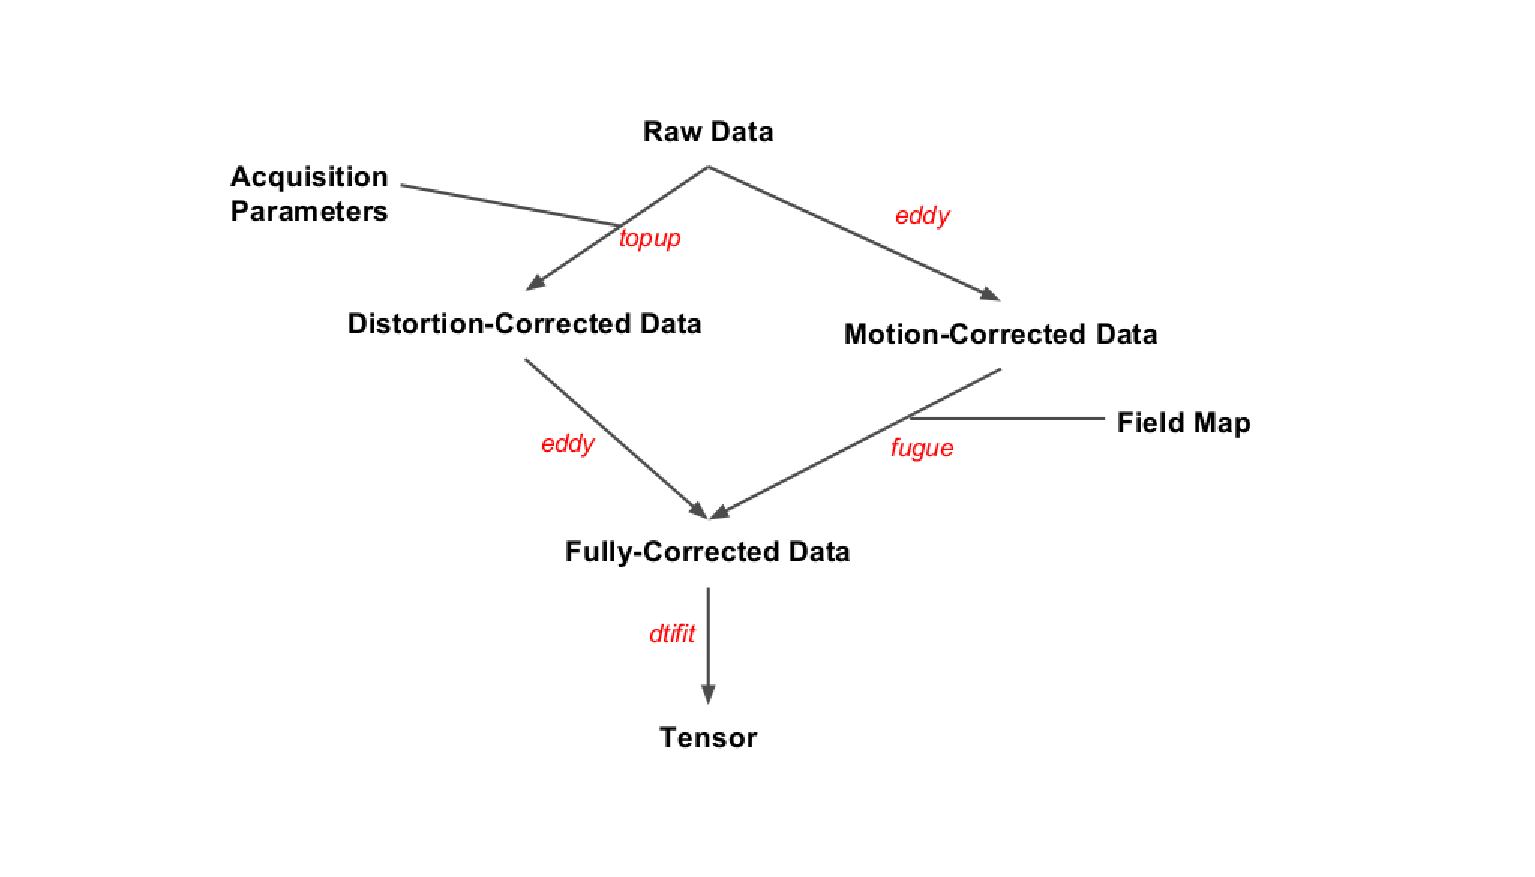
\includegraphics[width=\textwidth]{images/distcorr-flowchart.eps}
	\end{center}
	\caption{Flowchart of the Toy Makefile}
	\label{toy-example}
\end{figure}


If we were to implement this process in a \bashn{} script, the earlier
``upstream'' processes would need to be part of the conditional
block. An advantage of using \maken{} for workflows is that
\emph{only} the part that causes the ``split'' in the branching logic
needs to be surrounded by the if-then-else-end logic. Also note that
if we were using \texttt{topup} with a fieldmap, but for some reason
we wanted to do just the motion correction (like for QC, or for
debugging purposes), that unused ``branch'' of the makefile would be
available with a simple \texttt{make motion_corrected_dataset}
command. \newpage


Here's the full Makefile, located in
\texttt{dti_suceptibility_correction/subjects/fugue_DTI} and
\texttt{dti_suceptibility_correction/subjects/topup_DTI}. You can see
each of these files is in fact a symbolic link to the same file, located in
\texttt{dti_suceptibility_correction/lib/diffusion.Makefile}.

\setcounter{codehighlight}{0}
\begin{lstlisting}
	ifeq "$(origin MAKEPIPELINES)" "undefined"
	MAKEPIPELINES=/project_space/makepipelines
	endif

	PROJECT_DIR=$(MAKEPIPELINES)/dti_suceptibility_correction

	SDC_METHOD = $(shell if [ -f fieldmap.nii.gz ] ; then echo FUGUE; \
	                    elif [ -f acqparams.txt ] ; then echo TOPUP; \
	                    else echo FALSE ; fi)


	%*\lnote*NUM_DIFFUSION_VOLS =$(shell fslval raw_diffusion.nii.gz dim4 | tr -d '\040\011\012\015')


	%*\lnote*EDDY_ITERATIONS = 1
	TOPUP_MODE=fast
	ECHO_SPACING =.00072
	UNWARP_DIRECTION=y-

	.PHONY: clean tensor

	%*\lnote*mec_diffusion.nii.gz: raw_diffusion.nii.gz bval bvec brain_mask.nii.gz
		echo "0 1 0 0.072" > temp_acqparams.txt ;\
		for i in `seq 1 $(NUM_DIFFUSION_VOLS)`; do echo 1 >> temp_index.txt ; done ;\
		eddy --imain=raw_diffusion.nii.gz --mask=brain_mask.nii.gz \
			--index=temp_index.txt --acqp=temp_acqparams.txt --bvecs=bvec \
			--bvals=bval --out=mec_diffusion --niter=$(EDDY_ITERATIONS) \
			--verbose  ;\
		rm temp_acqparams.txt temp_index.txt

	%*\lnote*topup_results_movpar.txt: raw_diffusion.nii.gz acqparams.txt
		fslroi raw_diffusion.nii.gz S0_images.nii.gz 0 2 ;\
		topup --imain=S0_images --datain=acqparams.txt \
			--config=$(PROJECT_DIR)/lib/b02b0_$(TOPUP_MODE).cnf \
			--out=topup_results --fout=field_est --iout=unwarped_S0_images \
			--verbose

	ifeq ($(SDC_METHOD),TOPUP)
	sdc_mec_diffusion.nii.gz: raw_diffusion.nii.gz topup_results_movpar.txt index.txt
		eddy --imain=raw_diffusion.nii.gz --mask=brain_mask --acqp=acqparams.txt \
			--index=index.txt --bvecs=bvec --bvals=bval \
			--topup=topup_results \
			--out=sdc_mec_diffusion.nii.gz --niter=$(EDDY_ITERATIONS) \
			--verbose
		
	else ifeq ($(SDC_METHOD),FUGUE)
	sdc_mec_diffusion.nii.gz: mec_diffusion.nii.gz fieldmap.nii.gz
		fugue --loadfmap=fieldmap.nii.gz --dwell=$(ECHO_SPACING) \
			-i mec_diffusion.nii.gz -u sdc_mec_diffusion.nii.gz \
			--unwarpdir=$(UNWARP_DIRECTION) -v
	else
	$(error ERROR: neither fieldmap for FUGUE nor acquisition parameter file for TOPUP were found)
	endif

	tensor: sdc_mec_diffusion.nii.gz brain_mask.nii.gz bvec bval
		dtifit -k sdc_mec_diffusion.nii.gz -r bvec -b bval -m brain_mask -o dti

	clean:
		rm -f dti_* sdc_mec_diffusion.* mec_diffusion.* S0_images* \
		field_est.nii.gz topup_results* unwarped_S0_images.nii.gz

\end{lstlisting}


\lnum{1}\texttt{fslval} returns a trailing space as part of its output, which we pipe to \texttt{tr} for deletion.

\lnum{2}The settings here are for a quick test run for demonstration
purposes. For more accurate (but slower) processing,
\texttt{TOPUP_MODE} can be changed to 'accurate', and
\texttt{EDDY_ITERATIONS} can be increased to 5. Placing the settings
clearly in the Makefile makes it easy to extract them for quality
assurance reports. 

\lnum{3}In addition to running \texttt{eddy}, this recipe creates a simple acquisition parameters file and a simple index file (\texttt{eddy} requires that you supply one). This tells \texttt{eddy} that all the images were acquired with the phase encoding along the same direction. These files are deleted afterwards.

\lnum{4}The first two images are assumed to be the two non-diffusion weighted images (i.e. the $S _{0}$ images), with the phase encoding along different directions.


There are a few more files and commands here than in the toy example,
but the basic structure is the same. It's still missing some elements
of a full-featured DTI preprocessing pipeline (for example, unwarping
the brain mask, coregistration of the fieldmap with the diffusion
data, and rotation of the b-vectors), but this example illustrates how
using conditional statements in makefiles can make them more robust
and versatile.

\vspace{\baselineskip}
\hrule
\vspace{\baselineskip}

More information about the options and the formats of the files
supplied to \texttt{eddy}, \texttt{topup}, and \texttt{fugue} is
available on the
\href{http://fsl.fmrib.ox.ac.uk/fsl/fslwiki/FslOverview}{FSL website}.





 \clearpage \setcounter{codehighlight}{0}
\Echapter{Quantifying Arterial Spin Labeling Data}{Swati D. Rane}{srleven@uw.edu}
\label{chap:asl}
This is an example
of how to use a makefile to quantify cerebral blood flow (CBF) from
pseudo-continuous arterial spin labeling (pCASL) data. 

The code for this example is in
\texttt{\$MAKEPIPELINES/ASLTestsubject/S001/Makefile}. S001 is the
name of the subject and the folder name. In this example 
we assume we have one folder per subject. The folder name
reflects the subject name and contains the
\texttt{SUBJECTNAME_ASL.nii.gz} and \texttt{SUBJECTNAME_M0.nii.gz}
files. The ASL file contains alternating volumes from the control and
label acquisitions, where the odd volumes are control volumes and the even
volumes are the label volumes. The M0 file is a single 3D volume of
the reference proton density weighted image.

A unique feature of this example is that we have
performed surround subtraction in MATLAB to improve the 
signal-to-noise ratio of the ASL data.  We have included a standalone 
MATLAB application that can be installed with the necessary runtime binaries 
and libraries to complete this step. Note that this approach does not  
require you to have MATLAB installed on your computer. Similarly, if
you have a limited number of floating licenses available, deploying a
standalone MATLAB application does not require a floating license. 

If you are not at IBIC, before running this example you must install
the MATLAB runtime libraries and surround subtraction application as follows:
\\
Change directory to \texttt{ASLTestsubject/bin} and run the program
\texttt{SSInstaller_mcr.install} as shown in \autoref{bash:matlab}.
\begin{bash}{Installing MATLAB Runtime Libraries and surround
    subtraction application}{bash:matlab}
cd \$MAKEPIPELINES/ASLTestsubject/S001/Makefile\\
./SSInstaller_mcr.install
\end{bash}

\begin{figure}
\begin{center}
  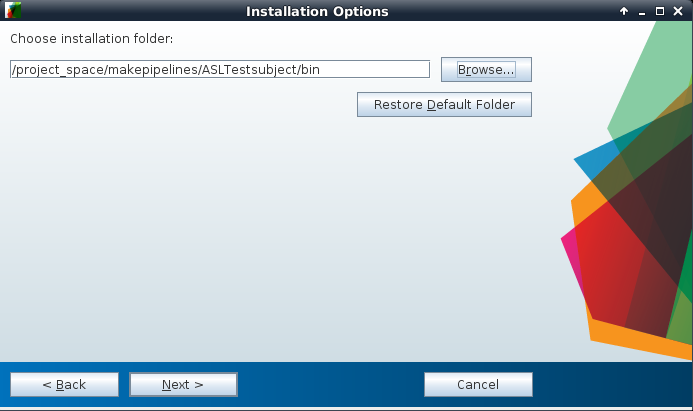
\includegraphics[scale=.6]{images/installApp2.png}
\caption{Entering location of installation folder for Surround 
  Subtraction standalone MATLAB application.}
\label{fig:ssinstall2}
\end{center}
\end{figure}

The installer will, perhaps after some delay, open a splash screen
with an opportunity to change connection settings. Just click next.
The next screens will prompt for a location for the installation folder
(see \autoref{fig:ssinstall2}). Enter the location of
\texttt{\$MAKEPIPELINES/ASLTestsubject/bin} whenever asked. Note that
here, the value of \texttt{MAKEPIPELINES} is set to
\texttt{/project_space/makepipelines}. In your environment this will
be different.
\clearpage

\begin{lstlisting}
	SHELL=/bin/bash

	%*\lnote*tau = 1.5
	pld = 1.525
	label_eff = 0.85
	T1b = 1.627
	lambda=0.9

	ifeq "$(origin MAKEPIPELINES)" "undefined"
	MAKEPIPELINES=/project_space/makepipelines
	endif

	PROJECT_HOME = $(MAKEPIPELINES)/ASLTestsubject/S001

	%*\lnote*#FSLDIR=/usr/share/fsl/5.0
	FSL_PATH = ${FSLDIR}/bin


	%*\lnote*MATLAB_PATH = $(MAKEPIPELINES)/ASLTestsubject/bin
	STD_BRAIN2mm = ${FSLDIR}/data/standard/MNI152_T1_2mm_brain.nii.gz
	STD_BRAIN2mm_MASK = ${FSLDIR}/data/standard/MNI152_T1_2mm_brain_mask.nii.gz
	STD_BRAIN2mm_GM = ${FSLDIR}/data/standard/tissuepriors/avg152T1_gray.img

	SUBJECT = $(shell basename ${PROJECT_HOME})	
\end{lstlisting}

\lnum{1}CBF quantification requires specific sequence parameters such as label duration (\texttt{tau}), post labeling delay (\texttt{pld}), longitudinal relaxation, T1 of blood (\texttt{T1b}). \texttt{label_eff} and \texttt{lambda} are constants defining the labeling efficiency for pCASL and the tissue-blood partition coefficient respectively. For convenience, we have predefined the paths for subject directory \texttt{PROJECT_HOME} as well as standard template brains and masks under \texttt{STD_BRAIN2mm}, \texttt{STD_BRAIN2mm_MASK}, and \texttt{STD_BRAIN2mm_GM}. 

\lnum{2}Because we have multiple versions of FSL installed, we set variables to describe what version of FSL we are using in the Makefile. 

\lnum{3} The MALTAB app is a \texttt{.mcr} file. Double clicking will open an installation window to copy the codes to a user-specified location. In this project, we have copied these files and folders in the \texttt{bin} directory under \texttt{ASLTestSubject}. This can serve as the common directory for all subjects. The \texttt{surround_subtraction.sh} is the shell file that calls \texttt{run_Surround_Subtraction.sh} generated by the MATLAB app. 
 
\begin{lstlisting}
	.PHONY =  all clean
	all:${SUBJECT}_CBF_MNI.nii.gz  QA/ASL.gif
	
	${SUBJECT}_mc_ASL.nii.gz: ${SUBJECT}_ASL.nii.gz ${SUBJECT}_M0.nii.gz
		${FSL_PATH}/mcflirt -in $< -reffile $(word 2,$^) -out $@;
\end{lstlisting}

In this segment of code, we motion correct the ASL data using MCFLIRT in FSL. Because the ASL and M0 data are acquired as separate scans, all ASL volumes are registered to the M0 volume. This is unlike the motion correction typically performed in BOLD fMRI where the central dynamic is considered as the reference volume. All remaining volumes are registered to this central volume.

\begin{lstlisting}
	#Implement surround subtraction for calculating differences in MATLAB
	%*\lnote*${SUBJECT}_DeltaM.nii.gz: ${SUBJECT}_mc_ASL.nii.gz 
		${MATLAB_PATH}/surround_subtraction.sh $< ${MATLAB_PATH} 
	
	%*\lnote*${SUBJECT}_CBF.nii.gz:${SUBJECT}_DeltaM.nii.gz ${SUBJECT}_M0.nii.gz;
		${FSL_PATH}/fslmaths $< -div $(word 2,$^) temp;\
		${FSL_PATH}/fslmaths temp -mul \
		$(shell echo "scale=5; 6000*${lambda};" | bc -l) temp ;\
		${FSL_PATH}/fslmaths temp -mul  \
		$(shell echo "scale=5; e(${pld}/${T1b});" | bc -l) temp;\
		${FSL_PATH}/fslmaths temp -div \
		$(shell echo "scale=5; 2*${label_eff}*${T1b}*(1-e(-${tau}/${T1b}));" \
		| bc -l) $@;\
		rm temp.nii.gz
\end{lstlisting}

In this section, we compute absolute values of CBF. \lnum{4} The \texttt{surround_subtraction.sh} script evaluates the dimensions of the ASL data (rows, columns, slices) and calls the MATLAB script via \texttt{run_Surround_Subtraction.sh}. \lnum{5} CBF is computed in ml/100gm/min, from the ASL white paper \citep{ASLdementia}. 

\begin{lstlisting}
	${SUBJECT}_CBF_MNI.nii.gz: ${SUBJECT}_M0.nii.gz ${SUBJECT}_CBF.nii.gz
		${FSL_PATH}/flirt -in $< -ref ${STD_BRAIN2mm} -out temp.nii.gz \
		-omat cbf_to_MNI.mat -bins 256 -cost corratio -searchrx -90 90 \
		-searchry -90 90 -searchrz -90 90 -dof 12  -interp trilinear;\
		${FSL_PATH}/flirt -in $(word 2, $^) -ref ${STD_BRAIN2mm} \
		-out temp.nii.gz -applyxfm -init cbf_to_MNI.mat;\
		${FSL_PATH}/fslmaths temp.nii.gz -mul ${STD_BRAIN2mm_MASK} $@;\
		rm temp.nii.gz
\end{lstlisting}

This portion of the Makefile registers the CBF map to MNI space and
removes background. We did not have a corresponding T1 image for this
ASL data. Hence we regististered the M0 image directly to the the
standard 2mm MNI template available in FSL. We then applied the
subsequent transformation matrix to the CBF map. 

Ideally, if a T1 image were available, this step would be
different. We would register the M0 image to the subject's native T1
image. The T1 image would be registered to the MNI template, and we
would combine the two transformation matrices to register the CBF map
to MNI space.

\begin{lstlisting}
	QA/ASL.png:${SUBJECT}_CBF_MNI.nii.gz
		mkdir -p ${PROJECT_HOME}/QA;\
		${FSL_PATH}/slicer $< -i 0 150 -a QA/ASL.png;\
		${FSL_PATH}/fslmaths ${STD_BRAIN2mm_GM} -thr 130 temp;\
		${FSL_PATH}/fslmaths $< -mas temp temp;\
		
		gm_cbf=`${FSL_PATH}/fslstats -t temp -M';\
		echo $$gm_cbf;\
		echo "---" > QA/ASL_QA.Rmd;\
		echo "output: html_document" >>QA/ASL_QA.Rmd;\
		echo "---" >> QA/ASL_QA.Rmd;\
		echo "# ASL QA" >> QA/ASL_QA.Rmd;\
		echo `<img src="../QA/ASL.png" width=900px; />' >> QA/ASL_QA.Rmd;\
		echo        >> QA/ASL_QA.Rmd;\
		%*\lnote*echo  `Typical GM CBF = 49(2) ml/100gm/min'  >> QA/ASL_QA.Rmd;\
		echo        >> QA/ASL_QA.Rmd;\
		echo  `This subject, GM CBF = '$$gm_cbf >> QA/ASL_QA.Rmd;\
		%*\lnote*R -e `library("knitr");knitr::knit2html("QA/ASL_QA.Rmd","QA/ASL_QA.html")'

\end{lstlisting}

In the last section, we make a QA report for the ASL quantification
process.  
\lnum{6} Typical CBF values in the gray matter in healthy
adults is 49 $\pm$ 2 ml/100gm/min and is provided as reference. This
value is lower than the standard 55 ml/100gm/min, because we did not
correct for partial volume effects. In this piece of code, we evaluate
CBF in the gray matter. Because no native T1 images are available for
this subject, we used the the standard 2mm resolution gray matter mask
available in FSL. As part of the QA, we generate an image of CBF maps
along the mid-sections in all three planes.

\lnum{7} The image for QA and the
CBF values (typical and measured) are embedded in a R markdown file
which is then knit to obtain an HTML report for every subject.

\begin{lstlisting}
	clean:
		rm -f $(wildcard [A-Z][0-9][0-9][0-9]_CBF*.nii.gz) \
		$(wildcard [A-Z][0-9][0-9][0-9]_Del*.nii.gz) dimen.txt;\
		rm  -f $(wildcard [A-Z][0-9][0-9][0-9]_mc_*.nii.gz) temp.nii.gz \
		cbf_to_MNI.mat ASL_QA.md;\
		rm -r QA

\end{lstlisting}

The final target \texttt{clean} removes intermediary NIFTI files and matrix or text files using wildcards. Preprocessed images generated for QA reports can also be cleaned up this way. 

 \clearpage \setcounter{codehighlight}{0}


\chapter{Processing Scan Data for a Single Test Subject}
\label{example:testsubject}
\section{Testsubject Main Makefile}
\label{example:testsubjectmakefile}

This is an example of a subject-specific makefile that includes
pipelines (written using \maken{}) that have been developed by several people to process different types of
subject-level MRI data. Because there is only one subject in
this example, this subject specific makefile is not a symbolic link,
as it is in the \texttt{oasis-longitudinal-sample-small} directory. 

The code for this example is in \texttt{\$MAKEPIPELINES/testsubject/test001/Makefile}. 

\setcounter{codehighlight}{0} % RESET THIS BEFORE EVERY LST LISTING
\begin{lstlisting}
	%*\lnote*.PHONY = etiv fast flex robex freesurferskullstrip 

	%*\lnote*FSL_DIR=/usr/share/fsl/5.0 

	STD_BRAIN=$(FSL_DIR)/data/standard/MNI152_T1_2mm.nii.gz 

	ifeq "$(origin MAKEPIPELINES)" "undefined"
	MAKEPIPELINES=/project_space/makepipelines 
	endif 

	%*\lnote*t1subj := $(shell pwd) 
	subject := $(notdir $(t1subj)) 

	PROJECT_HOME=$(MAKEPIPELINES)/testsubject/

	%*\lnote*include $(PROJECT_HOME)/lib/makefiles/help_system.mk 
	include $(PROJECT_HOME)/lib/makefiles/resting.mk 
	include $(PROJECT_HOME)/lib/makefiles/xfm.mk 
	include $(PROJECT_HOME)/lib/makefiles/fcconnectivity.mk 
	include $(PROJECT_HOME)/lib/makefiles/QA.mk 
	include $(PROJECT_HOME)/lib/makefiles/methodsgenerator.mk

	%*\lnote*export OMP_NUM_THREADS=1 

	SHELL=/bin/bash 

	%*\lnote*FLEXPATH=$(PROJECT_HOME)/bin/wmprogram/sb/cross_platform/scripts

\end{lstlisting}

\lnum{1} We begin by specifying our phony targets. These will be
defined later. 
\lnum{2} This line that sets \texttt{FSL_DIR} will be commented out in
your makefile, but you should find out where your version of FSL is
installed and make sure that it is correct. If we do not specify the
version of the programs that we run in a makefile, \maken{} will use
the individual's \texttt{PATH} variable to find them. Because
different people may have different \texttt{PATH} variables, this will
result in unpredictable results (the opposite of reproducibility!)
Recall that \maken{} inherits variables from your environment, and you
can override them by setting them.

\lnum{3} It is useful to have a variable to refer to the
subject. Here, we simply obtain the subject from the last part of the
directory name. This won't work for more complicated linking
structures as described in \nameref{sec:practicum2}. 

\lnum{4} We include lots of other makefiles that we need. This keeps
this makefile short and readable. 

\lnum{5} Certain programs do their own parallelization on computers
with multiple processing elements (cores). To turn this off, we
override the environment variable \texttt{OMP_NUM_THREADS}. This
allows us to use the \texttt{-j} flag to \maken{} to parallelize
execution of the entire makefile.

\lnum{6} FLEX is a program for white matter hyperintensity
quantification that we use for this project. This variable simply
specifies its location. If you do not have it installed you just won't
be able to run that part of the processing. It is not mandatory. 

\begin{lstlisting}
	 %*\lnote*FLAIR = $(shell if [ -f 00_NOFLAIR ] ; then echo false; else echo true; fi)

	 HAVET1 = $(shell if [ -f 00_NOT1 ] ; then echo false; else echo true; fi)

	 %*\lnote*ifeq ($(HAVET1),true)
	 %*\lnote*all: $(call print-help,all,Do skull stripping, etiv, HC volume calculation) T1_skstrip.nii.gz first etiv
	 else
	 all:  $(call print-help,all,Do skull stripping, etiv, HC volume calculation)
		@echo "Subject is missing T1 - nothing to do here."
	 endif
\end{lstlisting}

\lnum{7} In large and complicated studies, a certain type of image may
be missing, but this does not stop us from processing all the data
that we have. Here, we test for a FLAIR acquisition by looking for a
marker file in the directory called \texttt{00_NOFLAIR} (and similarly
for the T1). 

\lnum{8} Here we modify the target \texttt{all} depending on whether
or not the subject has a T1 image. We also use the help system
described in \nameref{sec:practicum4} to document what this target
does. 


\begin{lstlisting}
	T1_skstrip.nii.gz: T1.nii.gz 
		bet $< $@ -B

	robex: $(call print-help,robex,Alternate skull stripping with ROBEX) T1.nii.gz 
		$(PROJECT_HOME)/bin/ROBEX/runROBEX.sh T1.nii.gz T1_skstrip.nii.gz

	freesurferskstrip: $(call print-help,freesurferskullstrip, Alternate skull stripping with FreeSurfer) $(PROJECT_HOME)/freesurfer/$(subject)/mri/brain.mgz
		subj=$(subject) ;\
		mri_vol2vol --mov $(PROJECT_HOME)/freesurfer/$${subj}/mri/brain.mgz \
		--targ $(PROJECT_HOME)/freesurfer/$${subj}/mri/rawavg.mgz \
		--regheader --o brain-in-rawavg.mgz ;\
		mri_convert brain-in-rawavg.mgz brain-in-rawavg.nii.gz ;\
		fslreorient2std brain-in-rawavg.nii.gz T1_skstrip.nii.gz ;\
\end{lstlisting}

We have rules in this makefile for three methods of skull
stripping. The default is simply to call \texttt{bet} with the bias
correction option (which worked well on the data for the study this
makefile was modeled after). However, when this method did not work
well, we tried alternative methods using ROBEX and FreeSurfer. Note
that because the targets \texttt{robex} and \texttt{freesurferskstrip}
are phony, they can be created at any time and will always overwrite
\texttt{T1_skstrip.nii.gz}. 


\begin{lstlisting}
	etiv: $(call print-help, etiv, Estimation of ICV using enigma protocol) eTIV.csv

	brain_to_std.mat brain_to_std.nii.gz: T1_skstrip.nii.gz 
		flirt -in $< -ref $(STD_BRAIN) -omat $@ -out brain_to_std.nii.gz

	eTIV.csv: brain_to_std.mat
		%*\lnote*etiv=`$(PROJECT_HOME)/bin/mat2det brain_to_std.mat \
		| awk '{print $$2 }'` ;\
		echo  $(subject)","$$etiv > $@
\end{lstlisting}

We estimate intracranial volume (ICV) using the ENIGMA protocol (as described in
\nameref{sec:practicum3}). This approach calculates the inverse 
determinant of the linear transformation of the T1 image to standard
space. This is a scaling factor that we can multiply the volume of the
standard space brain by to obtain an estimated ICV volume. 

\lnum{9} Note that when calling the \texttt{mat2det} script and
echoing the results to a file, we need two dollar signs (\texttt{\$\$})
for every one that we intend to pass to the shell.  



\begin{lstlisting}
	 first: first_all_fast_firstseg.nii.gz T1.nii.gz hippo.csv

	 first_all_fast_firstseg.nii.gz : T1.nii.gz
		$(PROJECT_HOME)/bin/run_first_all_edit -s "L_Hipp,R_Hipp"  -d -i T1.nii.gz -o first

	 hippo.csv: first_all_fast_firstseg.nii.gz 
		rh=`fslstats $< -u 54 -l 52 -V|awk `{print $$2}'' ;\
		lh=`fslstats $< -u 18 -l 16 -V|awk `{print $$2}'' ;\
		echo $$lh $$rh > hippo.csv
\end{lstlisting}

We run FSL FIRST to calculate hippocampal volumes. We put these into a
comma separated value file to make it easy to remember how to extract
these numbers from the \texttt{first_all_fast_firstseg.nii.gz} and
check them (or include them in a QA report) although there is no
reason you could not write a separate program to gather them all.


\begin{lstlisting}
	 ifeq ($(FLAIR),true)
	 flex: $(call print-help,flex, Run flex for white matter hyperintensity quantification) flair.nii.gz flair_skstrip.hdr flair_skstrip_flwmt_lesions.hdr wmhstats.csv

	 flair_restore.nii.gz: flair.nii.gz
		fast -B -o flair -t 2 $<

	 flair_skstrip.nii.gz: flair_restore.nii.gz
		bet $< $@ -R

	 flair_skstrip.hdr: flair_skstrip.nii.gz 
		fslchfiletype ANALYZE $< $@

	 flair_skstrip_flwmt_lesions.hdr: flair_skstrip.hdr
		@echo "Flex processing " $< 
		$(FLEXPATH)/sb_flex -fl $< 

	 flair_skstrip_renamed.nii.gz: flair_skstrip.nii.gz
		cp $< $@

	 flair_wmh_mask.nii.gz: flair_skstrip_flwmt_lesions.hdr
		fslmaths $< -uthr 1 $@

	 else
	 flex:
		@echo No FLAIR, nothing to do
	 endif

	 wmhstats.csv: flair_skstrip_flwmt_lesions.hdr flair_skstrip_renamed.nii.gz
		@echo Writing wmhstats.csv 
		tot=`fslstats  flair_skstrip_renamed.nii.gz -V | awk `{print $$2}''; \
		wmh=`fslstats  flair_skstrip_flwmt_lesions.hdr -u 2 -V \
		| awk `{print $$2}'' ; \
		per=`echo $$wmh $$tot | awk `{print ($$1/$$2)*100}'' ; \
		echo  $(subject)", "$$wmh", " $$per >> $@ 
\end{lstlisting}

These are rules to run FLEX, a program for white matter hyperintensity
quantification from FLAIR images. This example comes from a multi-site
study where not all subjects obtained a viable FLAIR scan. If they do
have a FLAIR scan, we bias correct, skull strip, and process the data
using the program \texttt{sb_flex}.  The volume of white
matter hyperintensities (absolute volume and percent of skull stripped
brain) are written to \texttt{wmhstats.csv}. If we don't have a FLAIR
scan, there is nothing to do. You may not have FLEX installed on your
system in which case you can disregard this part of the makefile.


\begin{lstlisting}
	 archive:
		rm -rf flair_bc_*
		rm -rf flair_skstrip_axcor* flair_skstrip_flf_* flair_skstrip_WMT*
		rm -rf *~ \#* brain_to_std.nii.gz flair_skstrip.hdr flair_skstrip.img

	 clean:  $(call print-help,clean,Clean up everything from all makefiles) clean_rest clean_qa clean_transform clean_fcconnectivity clean_provenance
		rm -rf flair_skstrip* flair_pve* flair_restore* *~ wmhstats.csv eTIV.csv \
		brain_to_std* flair_mixeltype.nii.gz T1_skstrip_mask.nii.gz \
		first-L_Hipp* first-R_Hipp* T1_to_std_sub* \
		T1_skstrip.nii.gz hippo.csv first*
\end{lstlisting}

Finally, we define two targets to help us clean up. The first target,
\texttt{archive}, is intended to remove files that we don't need when
we intend to "tidy up". What we remove here is very subjective and
dependent upon the needs of the researchers. 

The second target, \texttt{clean} is intended to remove everything
from all makefiles to clean up everything. Note that \texttt{clean}
depends upon targets such as \texttt{clean_transform} and
\texttt{clean_rest} that are defined in the makefiles we have included
at the beginning. 

 \clearpage \setcounter{codehighlight}{0}
\section{Testsubject FreeSurfer}
\label{example:freesurfer}

This is an example of how to use a makefile to execute FreeSurfer in a cross-sectional context (in contrast to
\nameref{example:freesurfer}), which describes a longitudinal pipeline.  In addition, here we use FreeSurfer to
create a brain mask for skull stripping.

The code for this example is in \texttt{\$MAKEPIPELINES/testsubject/freesurfer/Makefile}.

\setcounter{codehighlight}{0} % RESET THIS BEFORE EVERY LST LISTING

\begin{lstlisting}
	ifeq "$(origin MAKEPIPELINES)" "undefined"
	MAKEPIPELINES=/project_space/makepipelines
	endif

	PROJHOME=$(MAKEPIPELINES)/testsubject 
\end{lstlisting}

This first section of the code looks to see if the environment variable
\texttt{MAKEPIPELINES} is set. This allows people who are not at IBIC
to override the default location of these files.

\begin{lstlisting}
	%*\lnote*include $(PROJHOME)/lib/makefiles/help_system.mk 

	%*\lnote*SUBJECTS=test001 

	export SUBJECTS_DIR=$(PROJHOME)/freesurfer 
	export FREESURFER_SETUP = /usr/local/freesurfer/stable5_3/SetUpFreeSurfer.sh 
	export RECON_ALL = /usr/local/freesurfer/stable5_3/bin/recon-all 
	export TKMEDIT = /usr/local/freesurfer/stable5_3/bin/tkmedit 
	QA_TOOLS=/usr/local/freesurfer/QAtools_v1.1 

	export SHELL=/bin/bash

	%*\lnote*outputstats=$(SUBJECTS:%=%/mri/aparc+aseg.mgz) $(SUBJECTS:%=%/mri/brainmask.mgz)
		$(SUBJECTS:%=%/mri/brainmask.nii.gz)

	%*\lnote*inputdirs = $(SUBJECTS:%=%)

	.PHONY: all clean qa freesurfer

	.SECONDARY: $(inputdirs) $(outputstats)
\end{lstlisting}

This portion of the Makefile defines key variables and targets. 
\lnum{1} We make use of the help system described in
\nameref{sec:practicum4}. 
\lnum{2} There is only one subject here, so for clarity we simply
write it out. However, in real life you would have many subjects, and
obtain them through a wildcard or from a file (see
\nameref{subsec:subjectlist}).
\lnum{3} We use pattern substitution to specify all of the output
targets we wish to create. These are the \texttt{aparc+aseg.mgz} file,
the \texttt{brainmask.mgz} file, and the brainmask converted to NIfTI
format (\texttt{brainmask.nii.gz}). Note that all of these files are
designated as SECONDARY targets so that they are not deleted at the end!
\lnum{4} We also use pattern substitution to set up the input directories.


\begin{lstlisting}
	 all: $(call print-help,all,Setup directories, Run Freesurfer, and Run QA) setup freesurfer qa

	 freesurfer: $(call print-help,freesurfer,Run FreeSurfer) $(outputstats)
\end{lstlisting}

The \texttt{all} and \texttt{freesurfer} targets here are documented
using the help system. 

\begin{lstlisting}
	%/mri/brainmask.mgz: %
		subj=$* ;\
		export FREESURFER_SETUP=$(FREESURFER_SETUP) ;\
		export WATERSHED_PREFLOOD_HEIGHTS='05 15 25 35' ;\
		rm -rf $${subj}/scripts/IsRunning.* ;\
		source $$FREESURFER_SETUP ;\
		export SUBJECTS_DIR=$(SUBJECTS_DIR) ;\
		recon-all  -subjid  $${subj} -multistrip -autorecon1 ;\
		height=`cat $${subj}/mri/optimal_preflood_height' ;\
		if [[ $$height == 05 ]]; then max=$$(( $$height + 5 )); \
		WATERSHED_PREFLOOD_HEIGHTS=`echo $$height $$max'; \
		else min=$$(( $$height - 5 )); max=$$(( $$height + 5 )); \
		WATERSHED_PREFLOOD_HEIGHTS=`echo $$min $$height $$max'; fi ;\
		export WATERSHED_PREFLOOD_HEIGHTS ;\
		recon-all -s $${subj} -multistrip -clean-bm -gcut
\end{lstlisting}

This rule creates the brain mask (in .mgz format). We use the
\texttt{-multistrip} flag to \texttt{recon-all} which allows us to try
multiple preflood heights, trying different thresholds
automatically. Then \texttt{recon-all} is continued using the optimal
height. Note that this approach will begin a separate process
for each preflood height (e.g., four processes). This makes it a bit
hard to run this pipeline on many brains in parallel. Normally, we use
this approach when we are processing subjects one at a time after they
have been scanned.

\begin{lstlisting}
	%/mri/brainmask.nii.gz: %/mri/brainmask.mgz
		export FREESURFER_SETUP=$(FREESURFER_SETUP) ;\
		source $$FREESURFER_SETUP ;\
		mri_convert $< $@
\end{lstlisting}
This rule converts the brain mask from \texttt{mgz} format to NIfTI format.

\begin{lstlisting}
	%/mri/aparc+aseg.mgz:  %/mri/brainmask.mgz 
		subj=$* ;\
		export FREESURFER_SETUP=$(FREESURFER_SETUP) ;\
		source $$FREESURFER_SETUP ;\
		export SUBJECTS_DIR=$(SUBJECTS_DIR) ;\
		recon-all -s $${subj} -autorecon2 -autorecon3 
\end{lstlisting}

This rule finishes the remaining stages of
\texttt{recon-all}. It depends upon the brain mask being generated
(the result of the previous rule).

\begin{lstlisting}
	 setup: $(call print-help,setup,Setup subject directories) $(inputdirs) 

	%:  $(PROJHOME)/%/T1.nii.gz 
		mkdir -p $@/mri/orig; \
		cp $^ $@/mri/orig; \
		cd $@/mri/orig; \
		mri_convert *nii.gz 001.mgz 
\end{lstlisting}

The \texttt{setup} target depends upon the T1 image in the subject
directory (here, in \texttt{\$PROJHOME}). It creates a FreeSurfer
style subject directory, copies the file there, and converts it to
NIfTI format. 

\begin{lstlisting}
	qa: $(call print-help,qa, Run QA - do this interactively with screensaver \
		shut off) $(inputdirs:%=QA/%)

	QA/%: %
		source $(FREESURFER_SETUP) ;\
		$(QA_TOOLS)/recon_checker -s $*
\end{lstlisting}

We run the FreeSurfer QA tools to generate images that we can put into
our own reports. One problem with QA is that the images cannot be
generated in parallel in batch. We include a warning in the help
system that they should be generated interactively without a
screensaver. 

\begin{lstlisting}
clean:
	echo rm -rf $(inputdirs)
\end{lstlisting}

Finally, we define a \texttt{clean} target to remove all processing
results. 
\clearpage \setcounter{codehighlight}{0}
\section{Testsubject Transformations}
%\def\sectionautorefname{Testsubject Transformations}
\label{example:testsubjectxfm}

This is an example of using a makefile to create a set of transformation matrices using different registration methods available in FSL. 

The code for this example is in \texttt{\$MAKEPIPELINES/testsubject/lib/makefiles/xfm.mk}. It is included by \texttt{\$MAKEPIPELINES/testsubject/test001/Makefile}. Therefore, certain variables that this example uses are defined there. This approach helps to organize multiple makefiles and reuse rules across projects.

\setcounter{codehighlight}{0} % RESET THIS BEFORE EVERY LST LISTING
\begin{lstlisting}
	.PHONY=clean_transform transforms 

	transforms:  $(call print-help,xfm,Create resting state to MNI transformations) xfm_dir xfm_dir/MNI_to_rest.mat
\end{lstlisting}

The first line defines two phony targets (clean\_transform and transforms). The \texttt{.PHONY} target can be set as many times as you need to, and note that each makefile included by \texttt{testsubject/test001/Makefile} defines phony targets. 

The second target, \texttt{xfm}, uses the \texttt{print-help} call introduced in \nameref{sec:practicum4} to document this main function, to create an MNI to resting state transformation.

\begin{lstlisting}
	xfm_dir:
	%*\lnote*	mkdir -p xfm_dir

	%*\lnote*xfm_dir/T1_to_MNI.mat: xfm_dir T1_skstrip.nii.gz 
		flirt -in T1_skstrip.nii.gz -ref $(STD_BRAIN) -omat $@
\end{lstlisting}

\lnum{1} We define a target to create a directory, \texttt{xfm_dir},
to hold all of our transformations. This is handy because it allows us to
reuse transformations for other analyses. We know that
the registrations saved here will be checked. 

\lnum{2} This is just a simple rule to call \texttt{flirt} to perform
linear registration of the skull stripped T1 image to the standard
brain. Note that the definition for \texttt{STD_BRAIN} comes from the
including makefile, as do the rules to create the file \texttt{T1_skstrip.nii.gz}.

\begin{lstlisting}
	rest_dir/rest_mc_vol0.nii.gz: rest_dir/rest_mc.nii.gz
		fslroi $< $@ 0 1

	xfm_dir/rest_to_T1.mat: rest_dir/rest_mc_vol0.nii.gz T1_skstrip.nii.gz
		mkdir -p xfm_dir ;\
		%*\lnote*epi_reg --epi=rest_dir/rest_mc_vol0.nii.gz --t1=T1.nii.gz \
		--t1brain=T1_skstrip.nii.gz --out=xfm_dir/rest_to_T1
		
\end{lstlisting}

These rules use FSL's \texttt{epi_reg} program to register the resting
state data to the subject's structural data. We noticed that
\texttt{epi_reg} used a lot of memory when running, limiting the
number of processors that we could use in parallel to preprocess
resting state data. \lnum{3} This requirement can be circumvented by using only
the first volume of the resting state data, obtained in the first
rule. 


\begin{lstlisting}
	xfm_dir/T1_to_rest.mat: xfm_dir/rest_to_T1.mat
		convert_xfm -omat $@ -inverse $<

	xfm_dir/MNI_to_T1.mat: xfm_dir/T1_to_MNI.mat
		convert_xfm -omat $@ -inverse $<

	xfm_dir/MNI_to_rest.mat:  xfm_dir/T1_to_rest.mat xfm_dir/MNI_to_T1.mat
		convert_xfm -omat xfm_dir/MNI_to_rest.mat \
		-concat xfm_dir/T1_to_rest.mat  xfm_dir/MNI_to_T1.mat
\end{lstlisting}
We obtain the T1 to resting matrix by inverting the resting to T1
matrix, and similarly for the MNI to T1 matrix. Finally, these
matrices are concatenated to create the final target,
\texttt{MNI_to_rest.mat}. Notice that everything else we needed was
automatically created as necessary to make this final target.


\begin{lstlisting}
	clean_transform: 
		rm -rf  xfm_dir 
\end{lstlisting}
Finally, we define a target to remove what we have created and clean
up. Notice that we call it \texttt{clean_transform}, rather than simply
\texttt{clean}, so that it does not override any other targets for
cleaning up that are included by the including Makefile.  \clearpage \setcounter{codehighlight}{0}
\section{Testsubject QA Makefile}
\label{example:testsubjectQA}

This is an example of using a makefile to create quality assurance (QA) images, and then generate a final QA report in HTML using R Markdown. 

The code for this example is in \texttt{testsubject/lib/makefiles/QA.mk}, and it is included by\linebreak \texttt{testsubject/test001/Makefile}.

\setcounter{codehighlight}{0} % RESET THIS BEFORE EVERY LST LISTING
\begin{lstlisting}
	%*\lnote*NIPYPATH=/usr/local/anaconda/bin
	FSL_DIR=/usr/share/fsl/5.0

	%*\lnote*.PHONY: TNSR MotionGraphs SkullstripQA QAReport

	%*\lnote*qa:   $(call print-help, qa, Create QA report) TSNR MotionGraphs SkullstripQA QAreport
\end{lstlisting}

\noindent\lnum{1} As is customary in a makefile, we first define paths
to locations that we want to refer to later on. \\
\lnum{2} Here, our phony targets are targets that are not actual files.\\
\lnum{3} This line tells the \maken{} help system what to do when you
are unsure of what this makefile does. Here, it will print out what
the \texttt{qa} target does (i.e., create a QA report). See \nameref{sec:practicum4} for more information about the help system. \\

\begin{lstlisting}
	%*\lnote*TSNR: QA/images/rest_tsdiffana.gif

	QA/images/%_tsdiffana.gif: rest.nii.gz
		%*\lnote*mkdir -p QA/images ;\
		%*\lnote*pngout= %*\`{}*echo $@|sed `s/gif/png/g'%*\`{}* ;\
		%*\lnote*$(NIPYPATH)/nipy_tsdiffana --out-file $$pngout $< ;\
		convert $$pngout $@ ;\
		rm -f $$pngout
\end{lstlisting}

\noindent\lnum{4} Our first target creates TSNR images for the QA. In this example, the phony target TSNR only wants \maken{} to create a single \texttt{gif} image. \\
\lnum{5} This line creates a directory called \texttt{QA/images} if it does not already exist. The \texttt{-p} flag tells \texttt{mkdir} not to throw an error if that directory exists, but create it if it does not.
\lnum{6} The variable \texttt{pngout} is defined to take the filename of your target and substitute \texttt{gif} with \texttt{png}.\\
\lnum{7} Subsequently, the code calls the script \texttt{nipy\_tsdiffana} which is located in the directory \texttt{\$(NIPYPATH)} you defined earlier.\\ The python script will generate a \texttt{png} image comprised of 4 graphs showing the scaled variance, slice-by-slice variance, scaled mean voxel intensity and the max/mean/min slice variation of your resting-state time series, as seen in the image below. \\

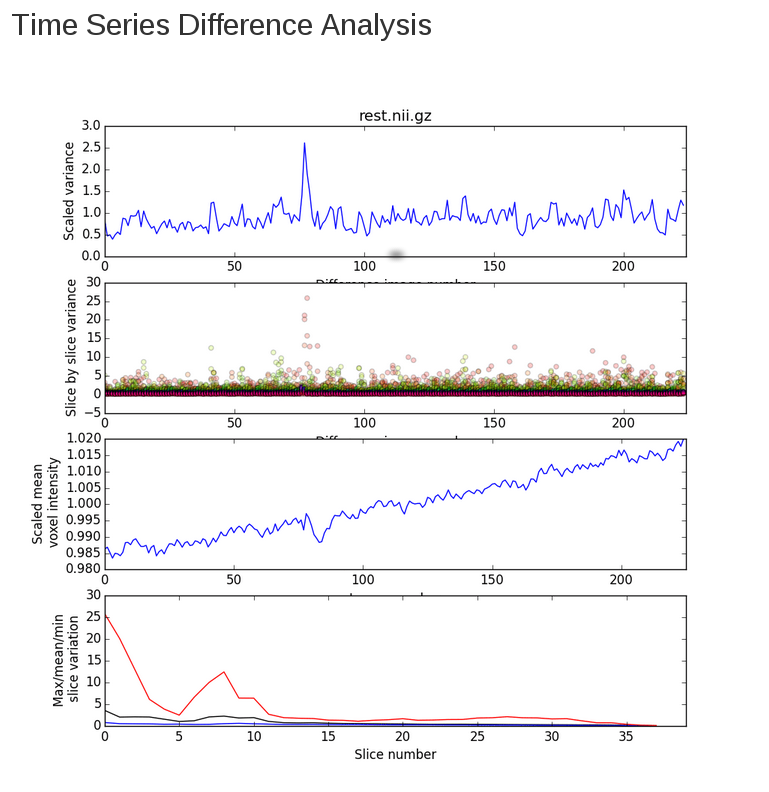
\includegraphics[scale=0.5]{images/QAtsdiffana.png}

\begin{lstlisting}
	MotionGraphs: QA/images/rest_MotionGraphRotations.gif 

	QA/images/rest_MotionGraphRotations.gif: rest_dir/rest_mc.nii.gz
		%*\lnote*$(PROJECT_HOME)/bin/R/MakingGraphs.Rscript  QA/images rest
\end{lstlisting}

\lnum{8}  \texttt{MakingGraphs.Rscript} is a R script that will generate 4 separate graphs for you: \\
	\tab 1. A motion rotations graph showing rotations along the x/y/z planes.\\
	\tab 2. A motion translations graph showing translations along the x/y/z planes.\\
	\tab 3. A framewise displacement (FD) graph to show displacement in mm across acquired volumes.\\
	\tab 4. A signal intensity (DVARS) graph to show signal intensity across acquired volumes.\\
	To understand the usage of an R script, it is usually necessary to look at the code itself. In this line, the R script called with the output directory \texttt{QA/images} as the first argument, followed by the prefix \texttt{rest} to be used for naming the output images.\\

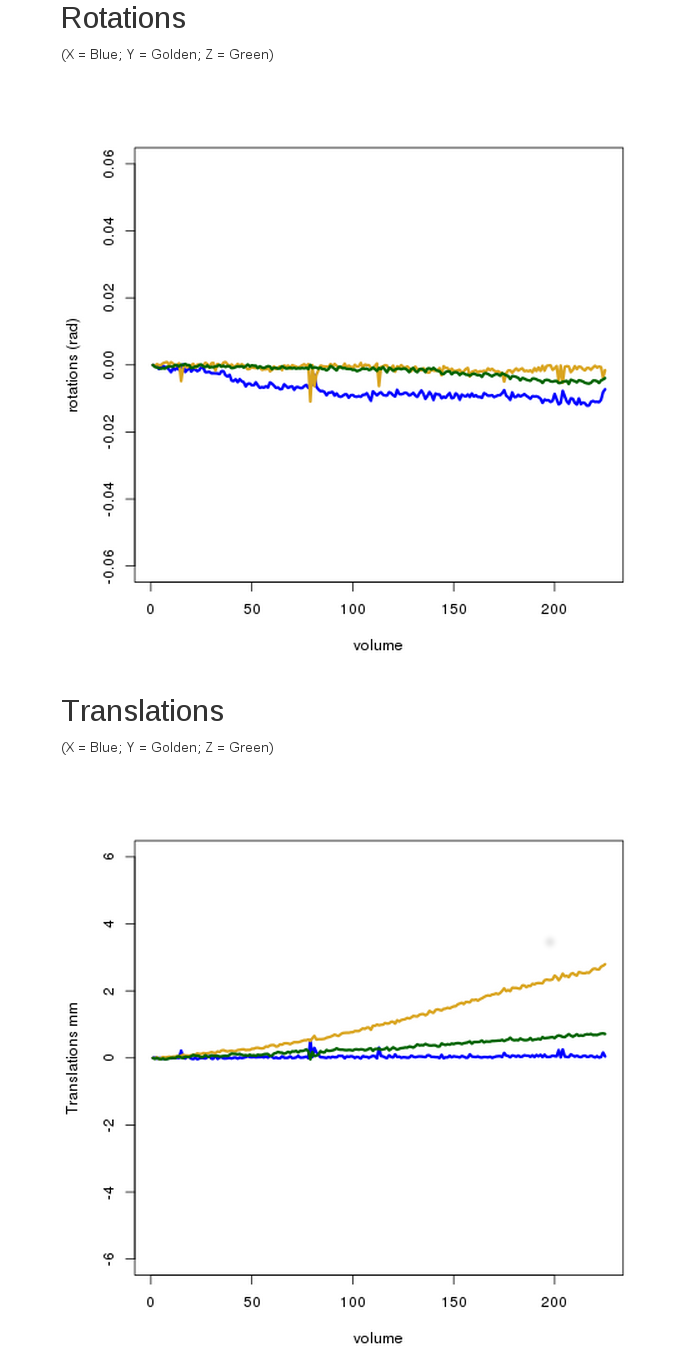
\includegraphics[scale=0.3]{images/QAmotion1.png}
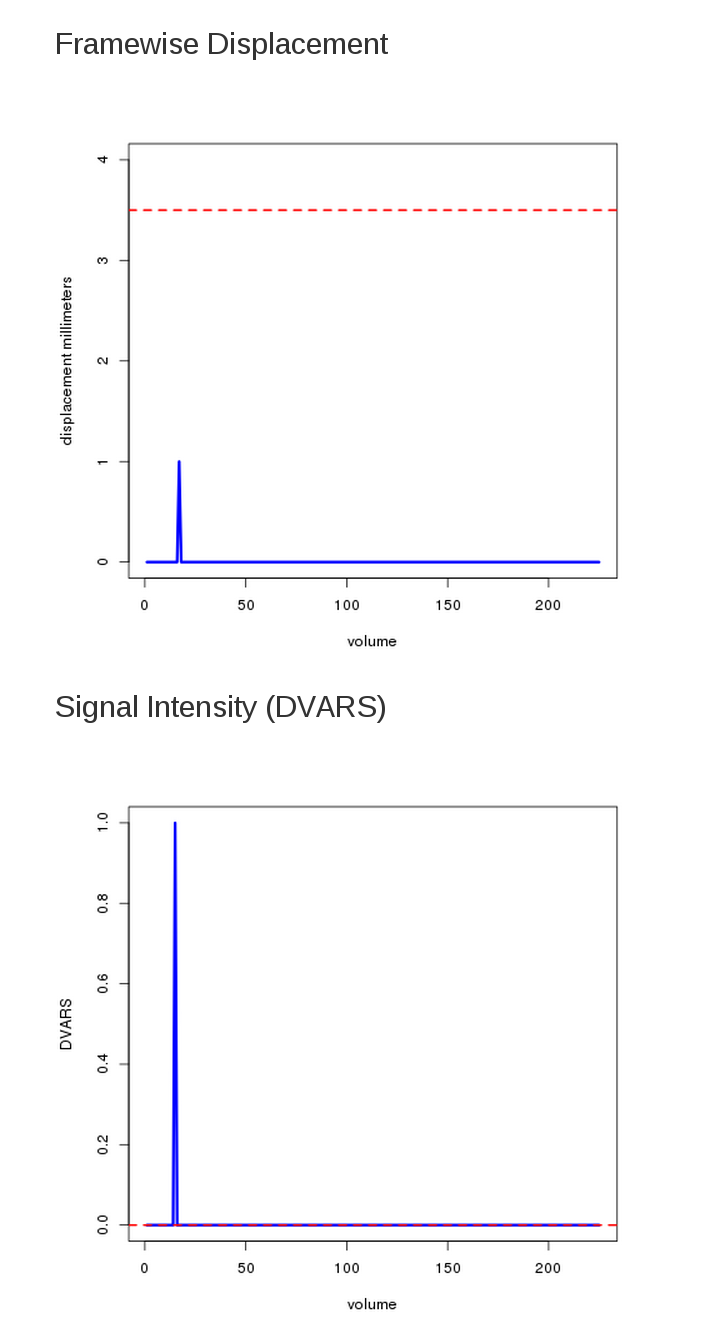
\includegraphics[scale=0.3]{images/QAmotion2.png}

\begin{lstlisting}
	SkullstripQA: QA/images/T1_skstrip.gif

	QA/images/T1_skstrip.gif: T1.nii.gz T1_skstrip_mask.nii.gz
		mkdir -p QA/images ;\
		%*\lnote*$(FSL_DIR)/bin/overlay 1 1 $< -a $(word 2,$^) 1 10 \
		rendered_T1_brain.nii.gz ;\
		%*\lnote*$(PROJECT_HOME)/bin/slices rendered_T1_brain.nii.gz \
		-o %*\`{}*dirname $@%*\`{}*/%*\`{}*basename $@ .gif%*\`{}*.png ;\
		%*\lnote*convert %*\`{}*dirname $@%*\`{}*/%*\`{}*basename $@ .gif%*\`{}*.png -resize 500 $@ ;\
		rm rendered_T1_brain.nii.gz ;\
		rm %*\`{}*dirname $@%*\`{}*/%*\`{}*basename $@ .gif%*\`{}*.png

\end{lstlisting}


To ensure that our skull-strip does not remove too much of the brain or too little of the skull, we can create an image to overlay the skull-stripped mask generated from \texttt{resting.mk} on top of the T1 brain. \\
\tab\lnum{9} FSL \texttt{overlay} is a tool that is used to overlay a 3D images over another. It is capable of overlaying a maximum of 2 images on top of a reference image. Type \texttt{overlay} into your command line to understand how it is used. In this line, we call \texttt{overlay}. The \texttt{1}s that are provided as arguments specify the color and output type of your overlay. The next argument is the background image, which in this case is the first dependency we have listed, i.e. \texttt{T1.nii.gz}. The \$\textasciicircum{} refers to this file. The final output image is called \texttt{rendered\_T1\_brain.nii.gz}. Again, to understand the flags, you must look at overlay's usage. \\
\lnum{10} FSL \texttt{slices} is a script that calls the FSL tool \texttt{slicer} to create an image consisting of 3 axial, 3 sagittal and 3 coronal slices. Here, we feed it the \texttt{rendered\_T1\_brain.nii.gz} file that we want FSL \texttt{slices} to use. The output will be a file called \texttt{QA/images/T1\_skstrip.png}. Instead of typing out the full name of the file, however, we simply provide the directory name and basename of our target and replace \texttt{.gif} with \texttt{.png}. \\
\lnum{11} Following this, we convert our PNG image into a GIF image, using ImageMagick's \texttt{convert} that performs the conversion and resizes the image.\footnote{This step was necessary in earlier versions of R Markdown that had trouble including PNG images, but may not be necessary for you.}\\

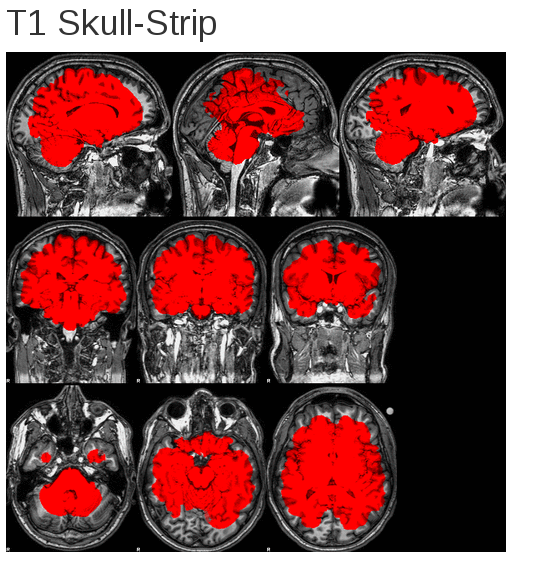
\includegraphics[scale=0.4]{images/QAskullstrip.png}

\begin{lstlisting}
	QAreport: QA/rest_Preprocessing.html 

	QA/rest_Preprocessing.html: $(PROJECT_HOME)/lib/Rmd/fMRI.Rmd TSNR MotionGraphs SkullstripQA
		%*\lnote*sed -e `s/SUBJECT/$(subject)/g' -e `s/TASK/rest/g' $(word 1,$^) > \
		QA/rest_Preprocessing.Rmd ;\
		%*\lnote*R -e `library("rmarkdown"); \
		rmarkdown::render("QA/rest_Preprocessing.Rmd")' ;\
		rm -f QA/rest_Preprocessing.Rmd QA/rest_Preprocessing.md
\end{lstlisting}


Finally, to generate our QA HTML report, we use R Markdown. We do this by writing a file called \texttt{fMRI.Rmd}, which is the first dependency listed here. The \texttt{fMRI.Rmd} file reads the QA images that were generated in the previous portions of this makefile to create a HTML page (see \nameref{sec:practicum4} for a brief explanation of what goes into a Rmd file and how to write one). \\
\lnum{12} In this line, we substitute pattern strings in the \texttt{fMRI.Rmd} file with variables that have been defined in the makefiles by using \texttt{sed}. \texttt{SUBJECT}, for instance, will be replaced with the \texttt{\$(subject)} variable defined in the main makefile \texttt{\$(PROJECT\_HOME)/test001/Makefile}. \texttt{TASK} will be replaced with \texttt{rest}, because we are only interested in looking at the QA report for resting-state functional scans for now. We can define another variable called \texttt{task} if we have several types of runs that we want to generate QA reports for (e.g., task runs or multiple resting state runs). Once the pattern strings have been substituted, the \texttt{fMRI.Rmd} file will be copied over to the \texttt{QA} directory and be renamed as \texttt{rest\_Preprocessing.Rmd}. \\
\lnum{13} This line tells R to load the `\texttt{rmarkdown}' library so that it can read the R Markdown file. R will then render \texttt{QA/rest\_Preprocessing.Rmd} to create your HTML report! \\

To view the full report, you can open the file \texttt{testsubject/test001/QA/rest_Preprocessing_example.html} in a browser.


\begin{lstlisting}
		clean_qa: 
		rm -rf QA
\end{lstlisting}

Finally, with other makefiles, we define a \texttt{clean} target specifically for QA. Because quality assurance is an intermediate step in the neuroimaging processing pipeline, we do not necessarily need to retain the QA images and reports once they have been checked.


 \clearpage \setcounter{codehighlight}{0}

\Echapter{Preprocessing Resting State Data}{Benjamin A. Korman}{bkorman@uw.edu}
\label{example:restingstate}
This is an example of how to use a makefile to preprocess functional resting state data. The pipeline incorporates typical preprocessing steps taken when preparing resting state data for analysis. This example includes motion and slice time acquisition correction, brain extraction, signal despiking, spatial smoothing and the calculation and removal of nuisance variables.

The code for this example is in \texttt{testsubject/lib/makefiles/resting.mk}. 

\setcounter{codehighlight}{0} % RESET THIS BEFORE EVERY LST LISTING
\begin{lstlisting}
	%*\lnote*cwd=$(shell pwd)

	SUBJECTS_DIR=$(PROJECT_HOME)/freesurfer
	SCRIPTpath=$(PROJECT_HOME)/bin

	FREESURFER_HOME=/usr/local/freesurfer/stable5_3

	%*\lnote*HWHM=3
	TR=2
	SLICEORDER=`ascending'
	NPC=5
	PCTVAR=0
	erosionfactor=1
\end{lstlisting}

\lnum{1} In any script or makefile, it is a good idea to set working
directory variables early on to ease the script writing process and to
avoid later confusion.  In this pipeline we have set a path variable
for our subject subdirectory \texttt{cwd} as well as for the
subdirectory that is home to the FreeSurfer pipeline's output
\texttt{SUBJECTS\_DIR}. In addition, we have set the variable
\texttt{SCRIPTpath} to the subdirectory home of additional scripts
that will be called during various preprocessing steps. \lnum{2}
Besides directory variables, it is helpful for us to set
processing-relevant variables which can be used throughout the
pipeline. Included here are variables for the half-width-half-maximum
(\texttt{HWHM}) kernel size needed for spatially smoothing the resting
state data, the time of repetition (\texttt{TR}) needed for slice time
correction, as well as the number of principal components
(\texttt{NPC}) and percent variance (\texttt{PCTVAR}) needed when
using principal component analysis to calculate regressors for
nuisance variables. Including these variables in the Makefile also
makes it easy to extract them for inclusion in a generated QA report.

\begin{lstlisting}
	%*\lnote*.PHONY: rest  Freesurfer_test regressors Run_aCompCor postregression clean_rest
	.SECONDARY:
\end{lstlisting}

\lnum{3} The targets listed in the \texttt{.PHONY} section are targets that do not correspond to actual files.   Some of these targets (ex. \texttt{regressors}, \texttt{postregression}) are intended to be used to process the resting state data in grouped steps whereas other \texttt{.PHONY} targets are related to cleanup or testing. One such target is \texttt{clean_rest} which may be called on to eliminate all of the pipeline's generated output when testing and debugging the pipeline.

	%*\lnote*rest: $(call print-help,rest,"Run resting state preprocessing pipeline") rest_dir rest_dir/rest_ssmooth.nii.gz Freesurfer_test xfm_dir/freesurfer_to_rest.mat regressors Run_aCompCor rest_dir/rest_abs_pc1.txt postregression

The \texttt{.PHONY} target \texttt{rest} is used here to easily invoke all preprocessing steps of the pipeline. This is the target we would use to completely preprocess a subject. It is documented using the help system (see \autoref{sec:practicum4}) and depends upon all preprocessing targets, described below.

\begin{lstlisting}
	%*\lnote*rest_dir/rest.nii.gz: rest.nii.gz 
		%*\lnote*echo "Setting up resting-state specific directory" 
		mkdir -p rest_dir ;\
		if [ ! -h rest_dir/rest.nii.gz ];\
		then \
		ln -s $(cwd)/rest.nii.gz rest_dir/rest.nii.gz;\
		fi;\
		if [ ! -h rest_dir/rest.nii.gz ];\
		then \
		ln -s $(cwd)/T1.nii.gz rest_dir/T1.nii.gz;\
		fi
\end{lstlisting}

\lnum{4} This target creates resting state specific subdirectory to keep our project directory clean and organized. We first create \texttt{rest_dir} and then create symbolic links within this directory to the files needed for preprocessing. The required files for resting state preprocessing in this pipeline include the subject's resting state NIfTI image and its corresponding T1 anatomical image.  \lnum{5} Before we do this, we echo (i.e., print to the screen) an informative message to provide progress information while the pipeline runs. Similar informational messages are distributed throughout the remainder of the makefile.

\begin{lstlisting}
	rest_dir/rest_mc.nii.gz: rest_dir/rest.nii.gz
		echo "Preprocessing RESTING scans..." ;\
		echo "Beginning motion correction for rest.nii.gz using 4dRegister" ;\
		%*\lnote*$(SCRIPTpath)/4dRegister.py --inputs $^ --tr $(TR) \
		--slice_order $(SLICEORDER) --time_interp True

\end{lstlisting}

Our first preprocessing step once a resting state-specific subdirectory has been created is to correct the resting state data for signal changes caused by motion and slice time acquisition. To do this we require the unprocessed resting state data, which is the sole dependency in this recipe.  \lnum{6} We will use \texttt{4dRegister.py}, a script provided by the Neuroimaging in Python (NIPY) community, to apply 4D motion and slice time correction simultaneously. The dependency \texttt{rest_dir/rest.nii.gz}, our input, is referred to as \texttt{\$\^} for short in the recipe. The resulting output will renamed with the  \texttt{_mc} extension to indicate that it has been motion corrected.

\begin{lstlisting}
	%*\lnote*rest_dir/rest_bet.nii.gz: rest_dir/rest_mc.nii.gz
		echo "Skull stripping resting data with FSL's BET" ;\
		bet $< $@ -F
\end{lstlisting}

\lnum{7} Following motion and slice time correction, we invoke FSL's BET with the \texttt{-F} flag to skullstrip the 4D resting state data. The output, referred to as \texttt{\$@} for short in the recipe, will be renamed  \texttt{_bet} to indicate that it has undergone brain extraction (aka skull stripping).

\begin{lstlisting}
	rest_dir/rest_despike.nii.gz: rest_dir/rest_bet.nii.gz
		echo "Despiking the functional data with AFNI" ;\
		%*\lnote*3dDespike -ssave spikiness -q $^ ;\
		3dAFNItoNIFTI despike+orig.BRIK ;\
		3dAFNItoNIFTI spikiness+orig.BRIK ;\
		echo "Renaming output, zipping it and deleting unnecessary despike files" ;\
		%*\lnote*mv despike.nii rest_dir/rest_despike.nii ;\
		mv spikiness.nii rest_dir/rest_spikiness.nii ;\
		rm -rf rest_dir/rest_despike.nii.gz rest_dir/rest_spikiness.nii.gz ;\
		gzip rest_dir/rest_despike.nii ;\
		gzip rest_dir/rest_spikiness.nii ;\
		rm -f despike+orig* ;\
		rm -f spikiness+orig*
\end{lstlisting}

\lnum{8} After skullstripping the brain, we perform voxel-wise despiking with AFNI to reduce noise caused by framewise displacement. \lnum{9} In addition to our despiked resting state output, a list of "spikiness" values is produced. These are renamed to \texttt{rest_despike.nii.gz} and \texttt{rest_spikiness.nii.gz} respectively. These output files are then compressed to save space while the original output files are removed.

\begin{lstlisting}
	%*\lnote*rest_dir/rest_ssmooth.nii.gz: rest_dir/rest_despike.nii.gz
		echo "Smoothing resting date with FSL's SUSAN" ;\
		susan $^ -1.0 $(HWHM) 3 1 0 $@
\end{lstlisting}

\lnum{10} Once the resting state data has been despiked it is ready to be spatially smoothed. To do this we use FSL's SUSAN with a 3D smoothing kernel 3mm in size. We rename our output with the  \texttt{_ssmooth} extension to indicate that it has been spatially smoothed.

\begin{lstlisting}
	%*\lnote*Freesurfer_test: $(SUBJECTS_DIR)/$(subject)/mri/brainmask.mgz 
			$(SUBJECTS_DIR)/$(subject)/mri/aparc+aseg.mgz

	%*\lnote*xfm_dir/rest_to_freesurfer.mat: rest_dir/rest_despike.nii.gz 
				$(SUBJECTS_DIR)/$(subject)/mri/aparc+aseg.mgz
		mkdir -p xfm_dir ;\
		source /usr/local/freesurfer/stable5_3/SetUpFreeSurfer.sh ;\
		export SUBJECTS_DIR=$(SUBJECTS_DIR) ;\
		fslroi rest_dir/rest_despike.nii.gz rest_dir/rest_despike_vol0 0 1 ;\
		bbregister --s $(subject) --mov rest_dir/rest_despike_vol0.nii.gz \
		--reg xfm_dir/rest_to_freesurfer.dat --init-fsl --bold \
		--o xfm_dir/rest_to_freesurfer.nii.gz \
		--fslmat xfm_dir/rest_to_freesurfer.mat

	%*\lnote*xfm_dir/freesurfer_to_rest.mat: xfm_dir/rest_to_freesurfer.mat
			convert_xfm -omat $@ -inverse $<
\end{lstlisting}

\lnum{11} To proceed with the calculation and removal of nuisance regressors from our spatially smoothed resting state data we first need to check whether the necessary FreeSurfer output files are available. This is because our estimation of background noise in the data will require white matter and cerebrospinal fluid masks which are created from the output of FreeSurfer's \texttt{recon-all} segmentation process. We normally run FreeSurfer separately, because it takes a lot longer to run than the resting state preprocessing. This target depends upon the FreeSurfer results \texttt{brainmask.mgz} and \texttt{aparc+aseg.mgz}. If these do not exist, no processing that depends upon this target can occur. Because the target \texttt{Freesurfer_test} is not an existing file (and will not at any point be created) it is included in the \texttt{.PHONY} section located above.

\lnum{12} Once we are certain that the necessary files exist in our FreeSurfer directory, we create a directory (\texttt{xfm_dir}) in which to keep all of our data transformations. Then, using \texttt{fslroi}, we select the first volume of our despiked resting state data (\texttt{rest_despike_vol0}) as input for FreeSurfer's \texttt{bbregister}. BBregister is used to perform within-subject, cross-modal rigid registration. \lnum{13} After registering the despiked data in FreeSurfer space we must transform this registration back into resting state space. This is because FreeSurfer space is unique and the pipeline will encounter problems if attempting to directly register images from FreeSurfer space to standard (i.e. MNI) space.

\begin{lstlisting}
	%*\lnote*regressors: rest_dir/fs_wMmask.nii.gz rest_dir/fs_csf_mask.nii.gz 
					rest_dir/rest_wm.nii.gz rest_dir/rest_csf.nii.gz

	%*\lnote*rest_dir/fs_wm_mask.nii.gz: $(SUBJECTS_DIR)/$(subject)/mri/aparc+aseg.mgz
		source /usr/local/freesurfer/stable5_3/SetUpFreeSurfer.sh ;\
		export SUBJECTS_DIR=$(SUBJECTS_DIR) ;\
		mri_binarize --i $^ --o $@ --erode 1 --wm

	rest_dir/fs_csf_mask.nii.gz: $(PROJHOME)/freesurfer/$(subject)/mri/aparc+aseg.mgz
		source /usr/local/freesurfer/stable5_3/SetUpFreeSurfer.sh ;\
		export SUBJECTS_DIR=$(SUBJECTS_DIR) ;\
		mri_binarize --i $^ --o $@ --erode 1 --ventricles
		
	%*\lnote*rest_dir/rest_wm.nii.gz: rest_dir/fs_wm_mask.nii.gz rest_dir/rest_despike.nii.gz 
				xfm_dir/freesurfer_to_rest.mat
		flirt  -ref $(word 2,$^) -in $(word 1,$^) -out $@ -applyxfm \
		-init $(word 3,$^) ;\	
		fslmaths $@ -thr .5 -bin $@

	rest_dir/rest_csf.nii.gz: rest_dir/fs_csf_mask.nii.gz rest_dir/rest_despike.nii.gz 
				xfm_dir/freesurfer_to_rest.mat
		flirt  -ref $(word 2,$^) -in $(word 1,$^) -out $@ -applyxfm \
		-init $(word 3,$^) ;\
		fslmaths $@ -thr .3 -bin $@
\end{lstlisting}

\lnum{14} The target \texttt{regressors} is included here for ease of use if one wanted to specifically create or recreate binarized masks from FreeSurfer's white matter and ventricle segmentations. \lnum{15} We binarize and extract white matter and ventricle masks. \lnum{16} We register the despiked resting state data to the white matter and CSF masks using  FSL's FLIRT.  Note that in the recipe the \texttt{\$(word \#, \$\^{})} refers to a dependency in the dependency list. The first dependency may be referenced in the recipe as \texttt{\$(word 1, \$\^{})}, the second \texttt{\$(word 2, \$\^{})}, and so forth.

\begin{lstlisting}
	%*\lnote*Run_aCompCor: rest_dir/rest_wm.txt rest_dir/rest_csf.txt

	rest_dir/rest_wm.txt: rest_dir/rest_despike.nii.gz rest_dir/rest_wm.nii.gz
		fslmaths rest_dir/rest_despike.nii.gz -mas rest_dir/rest_wm.nii.gz rest_dir/rest_wm_ts.nii.gz ;\
		%*\lnote*Rscript  $(SCRIPTpath)/aCompCor.R rest_dir/rest_wm_ts.nii.gz $(NPC) $(PCTVAR) ;\
		convert rest_dir/rest_wm_ts_VarianceExplained.png \
		rest_dir/rest_wm_ts_VarianceExplained.gif ;\
		rm rest_dir/rest_wm_ts_VarianceExplained.png ;\
		mv rest_dir/rest_wm_ts_pc.txt $@

	rest_dir/rest_csf.txt: rest_dir/rest_despike.nii.gz rest_dir/rest_csf.nii.gz
		fslmaths rest_dir/rest_despike.nii.gz -mas rest_dir/rest_csf.nii.gz rest_dir/rest_csf_ts.nii.gz ;\
		Rscript  $(SCRIPTpath)/aCompCor.R rest_dir/rest_csf_ts.nii.gz $(NPC) \
		$(PCTVAR) ;\
		convert rest_dir/rest_csf_ts_VarianceExplained.png \
		rest_dir/rest_csf_ts_VarianceExplained.gif ;\
		rm rest_dir/rest_csf_ts_VarianceExplained.png ;\
		mv rest_dir/rest_csf_ts_pc.txt $@
		
	%*\lnote*rest_dir/rest_abs_pc1.txt: rest_dir/rest_mc.nii.gz
		echo "Creating list of motion regressors using MotionRegressorGenerator.py" ;\
		$(SCRIPTpath)/MotionRegressorGenerator.py -i rest_dir/rest.par \
		-o rest_dir/rest
		
	%*\lnote*rest_dir/rest_nuisance_regressors.txt: rest_dir/rest_csf.txt rest_dir/rest_wm.txt rest_dir/rest_abs_pc1.txt
		echo "Combine lists of motion regressors into one text file" ;\
		paste $(word 1,$^) $(word 2,$^) $(word 3,$^) rest_dir/rest_rel_pc1.txt \
		> $@
\end{lstlisting}

Once we have registered the despiked resting state data to the white matter and CSF masks, we need to compute nuisance regressors. \lnum{17} The target \texttt{Run_aCompCor} depends upon these regressors and is a convenience target. \lnum{18} The R script \texttt{aCompCor} calculate nuisance regressors from the masked resting state data. This script can extract a set number of principal components \texttt{NPC} or by setting a specific percent of variance \texttt{PCTVAR} that should be explained by the principal components included in the analysis. In this example we use 5 principal components. 
 \lnum{19}  A python script named \texttt{MotionRegressorGenerator}, located in the \texttt{bin} directory, is also called in this pipeline to calculate nuisance regressors from motion parameters. \lnum{20} The nuisance regressors generated during this step are then combined with the nuisance regressors calculated by \texttt{aCompCor} into a single text file. 

\begin{lstlisting}
	%*\lnote*postregression: rest_dir/rest_designrange.txt rest_dir/rest_postregression.nii.gz
		echo "Regressing motion artifacts out of resting-state data"

	%*\lnote*rest_dir/rest_designrange.txt: rest_dir/rest_nuisance_regressors.txt
		Rscript $(SCRIPTpath)/rangeArray.R $< $@

	%*\lnote*rest_dir/rest_postregression.nii.gz: rest_dir/rest_ssmooth.nii.gz rest_dir/rest_nuisance_regressors.txt rest_dir/rest_designrange.txt
		npc=%*\`{}*awk `{print NF}' $(word 2, $^) | sort -nu | tail -n 1%*\`{}* ;\
		npts=%*\`{}*wc -l $(word 2, $^)%*\`{}* ;\
		echo "/NumWaves $$npc" >  rest_dir/rest_regressors.feat.mat ;\
		echo "/NumPoints $$npts" >> rest_dir/rest_regressors.feat.mat ;\
		echo "/PPheights " %*\`{}*cat $(word 3, $^)%*\`{}* >> \
		rest_dir/rest_regressors.feat.mat ;\
		echo "/Matrix" >> rest_dir/rest_regressors.feat.mat ;\
		cat $(word 2, $^) >> rest_dir/rest_regressors.feat.mat ;\
		fsl_regfilt -i  rest_dir/rest_ssmooth.nii.gz \
		-d rest_dir/rest_regressors.feat.mat  \
		-f %*\`{}*seq -s, 1 1 $$npc%*\`{}* -o $@
		
	%*\lnote*rest_dir/rest_outliers_dvars_vals.txt: rest_dir/rest_mc.nii.gz
			$(PROJECT_HOME)/bin/motion_outliers -i $^ \
			-o rest_dir/rest_outliers_dvars.txt \
			-s rest_outliers_dvars_vals.txt --dvars --nomoco
		
	rest_dir/rest_outliers_fd_vals.txt: rest.nii.gz
			$(PROJECT_HOME)/bin/motion_outliers -i $^ \
			-o rest_dir/rest_outliers_fd.txt \
			-s rest_outliers_fd_vals.txt --fd
\end{lstlisting}

Once the nuisance regressors have been calculated and combined into a single file, the next step is to remove them from the data. \lnum{21} This portion of the pipeline may be called specifically using the target \texttt{postregression}. \lnum{22} To regress out nuisance variables, we create a little FEAT design matrix and run \texttt{fsl_regfilt}. We calculate the range of the included nuisance regressors using the R script \texttt{rangeArray.R}. \lnum{23} Finally, we denoise the data by regressing out the nuisance regressors using simple ordinary least squares regression with FSL. \lnum{24} It may also be helpful to create text files listing motion outlier volumes based on dvars (RMS intensity differences in images between timepoints) or framewise displacement (fd). 

\begin{lstlisting}
	clean_rest:
		echo "Removing all output files except for freesurfer transforms" ;\
		rm -rf rest_dir
\end{lstlisting}

Lastly, we create a target to remove all files created by the pipeline. This is particularly useful when testing and debugging the pipeline. When called, this target will simply remove the \texttt{rest_dir} directory and all files located within it; in other words, everything that we have created with this Makefile.


 \clearpage  \setcounter{codehighlight}{0}
\Echapter{Generating A Methods Section}{Benjamin A. Korman}{bkorman@uw.edu}
\label{sec:provenance}
This is an example of how to use a makefile to automatically generate a methods section. Using a makefile to generate methods sections saves time and limits human error when reporting MRI acquisition and preprocessing parameters by obtaining the necessary values directly from the image source data, the computer system, and the processing pipelines themselves. This is an example of how we handle provenance --- we generate a human-readable description of the pipelines while saving information about the versions of the programs used to generate them. 

We do this in two steps. First, important parameters are written to a comma-separated value (CSV) file. These are extracted from wherever appropriate for the study using a \bashn{} shell script. For example, versions of tools such as FSL and AFNI can be obtained from the system. Imaging acquisition parameters can be obtained from the PAR file (a Philips human-readable parameter file), or the DICOMs, or any other exported parameter specification file appropriate to your study. Parameters that are used in the processing pipelines themselves can be obtained from those makefiles. After the CSV file is complete, we render an R Markdown file that loads those values and generates an HTML report. We include PubMed links to references in the R Markdown file so that, if necessary, the links can be used to import bibliographic records into bibliographic software databases. 

The code for this example is in \texttt{testsubject/lib/makefiles/methodsgenerator.mk}.  This example builds upon the other processing pipelines in place for \texttt{testsubject}, \texttt{dti_susceptibility_correction}, and \texttt{ASLTestsubject}. It describes the resting state processing pipeline in \nameref{example:restingstate}, the DTI susceptibility-correction pipeline in \nameref{chap:dti}, and the ASL processing pipeline in \nameref{chap:asl}.

\begin{lstlisting}
	%*\lnote*rs_parsource=$(wildcard parrecs/*REST*.PAR)
	t1_parsource=$(wildcard parrecs/*MPRAGE*.PAR)
	dti_parsource=$(wildcard parrecs/*DTI*.PAR)
	asl_parsource=$(wildcard parrecs/*ASL*.PAR)
\end{lstlisting}

This makefile begins by \lnum{1} searching for and selecting the PAR source files from which the makefile will acquire the majority of the generated methods section's parameter values. Because the naming conventions for the PAR files do not often follow a specific pattern, we use a wildcard to search for a string we are sure will be in the file name. 

\begin{lstlisting}
	%*\lnote*rs_framewisedisplacement="\#"
	rs_accelerationfactor="\#"
	t1_shotinterval="\#"
	dti_accelerationfactor="\#"
	asl_invertpulse1="\#"
	asl_invertpulse2="\#"
	asl_labelduration="\#"
	asl_postlabeldelay="\#"
	asl_M0_repetitiontime="\#"
\end{lstlisting}


\lnum{2} Not all of the necessary parameter values are available in PAR files, so there are few parameters that must be set (by replacing the \#'s specified for these values). Here we wish to report framewise displacement and acceleration factor used during resting-state data acquisition as well as the shot interval during the T1 anatomical scan acquisition along with parameters important for diffusion tensor imaging (DTI) and arterial spin labeling (ASL) processing. This makefile currently reports parameters important to resting-state, DTI, and ASL data and preprocessing but may be expanded to include other MRI techniques as well (e.g. voxel-based morphometry and susceptibility-weighted imaging).


\begin{lstlisting}
	%*\lnote*.PHONY: provenance clean_provenance
	.SECONDARY:
	
	%*\lnote*provenance: $(call print-help,provenance,"Automatically generate a methods section") provenancedir provenance/parameter_table.csv provenance/Methods_Generator.html
\end{lstlisting}

\lnum{3} The targets listed in the \texttt{.PHONY} section are targets that do not correspond to actual files. The target \lnum{4} \texttt{provenance} may be called to undertake all necessary steps towards creating an automated methods section while the target \texttt{clean_provenance} may be invoked to eliminate all of the makefile's generated output, useful for testing and debugging purposes.

\begin{lstlisting}
	%*\lnote*provenancedir: 
		echo "Creating provenance directory" ;\
		mkdir -p provenance
		
	%*\lnote*provenance/parameter_table.csv: provenancedir $(rs_parsource) $(t1_parsource) $(dti_parsource) $(asl_parsource)
		echo "Creating parameter table" ;\
		bash $(PROJECT_HOME)/bin/Methods_Generator.sh  $(rs_parsource) $(t1_parsource) $(dti_parsource) $(asl_parsource) $(rs_framewisedisplacement) $(rs_accelerationfactor) $(t1_shotinterval) $(dti_accelerationfactor) $(asl_invertpulse1) $(asl_invertpulse2) $(asl_labelduration) $(asl_postlabeldelay) $(asl_M0_repetitiontime) > $@
\end{lstlisting}

\lnum{5} This target creates a data provenance subdirectory to keep our project directory clean and organized. The files generated by this makefile will be stored in this folder. \lnum{6} Once a methods specific subdirectory has been created it is time to extract the parameter values we wish to include in our methods section from their respective PAR files and tabulate them appropriately. This is done by \lnum{7} calling a \bashn{} script which generates a table including the parameters' name (both an abbreviated form as well as a long form), value, and unit of measurement if applicable.

\begin{lstlisting}
	provenance/Methods_Generator.html: provenance/parameter_table.csv
		echo "Creating methods section html file" ;\
		cd provenance ;\
		cp $(PROJECT_HOME)/lib/Rmd/Methods_Generator.Rmd . ;\
		Rscript -e `library("rmarkdown"); \
		rmarkdown::render("Methods_Generator.Rmd")'
\end{lstlisting}

Using the \texttt{parameter_table.csv} file created in the previous step, an R script is called to incorporate the necessary parameter values into a model methods section R Markdown (.Rmd) file. One thing that is a little frustrating about R Markdown is that it will look for files in the directory in which it is located. This is why we first copy it to the \texttt{provenance} subdirectory. The R Markdown file then looks for the CSV file in the current working directory, with no need to pass paths back and forth between programs. 

The outputted methods section HTML file can be viewed in any web browser. \autoref{fig:methods} shows the R Markdown code that is processed (on the left) to generate the HTML report (on the right). The R Markdown code is very simple. The first ``chunk'' of code reads in the CSV file and uses the short variable names to construct a variety of variables for the value of the parameter, its full name, and the units. These are accessed in the text description of the protocol with the syntax \texttt{`r variablename'}. For more information about how to write reports with R Markdown, see their excellent \href{http://rmarkdown.rstudio.com}{documentation}. 

\begin{lstlisting}
	clean_provenance:
		echo "Removing provenance directory" ;\
		rm -r provenance
\end{lstlisting}

Lastly, we create a target to remove all files created by this makefile. When called, this target will simply remove the \texttt{provenance} directory and all files located within it.



\begin{figure}
	\begin{center}
		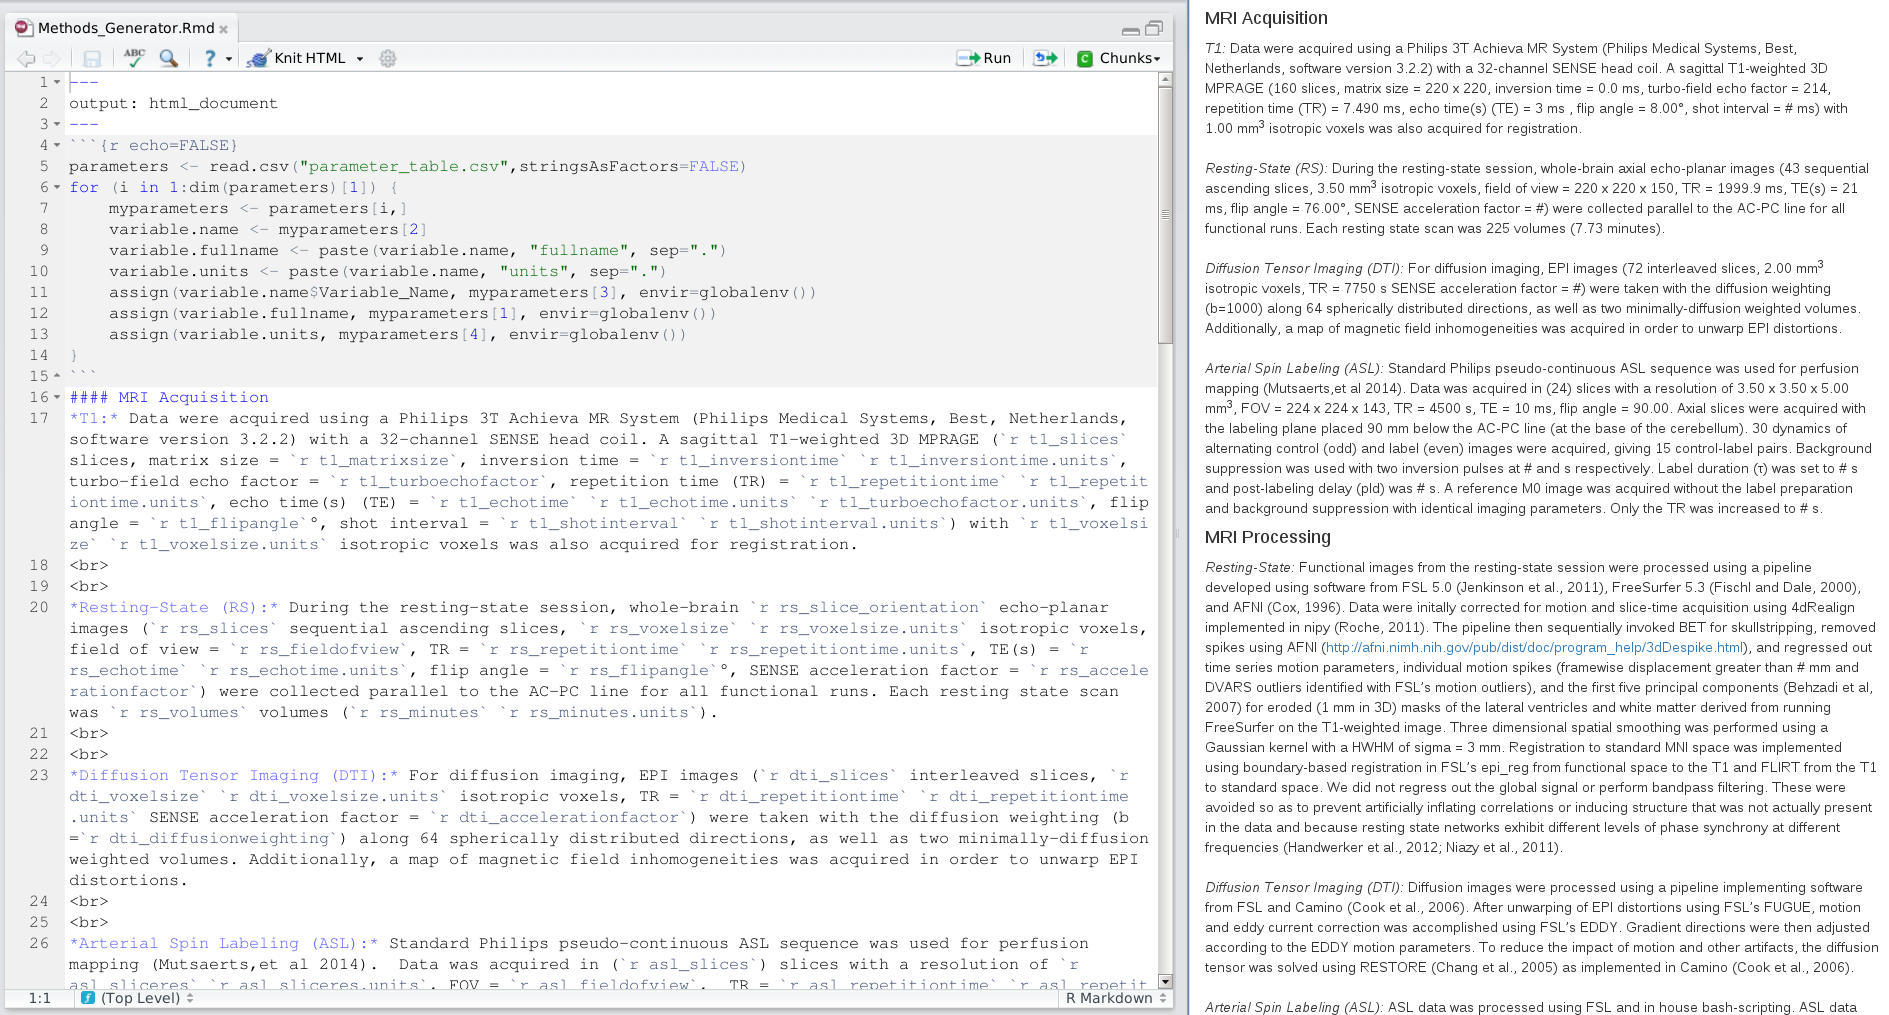
\includegraphics[width=7in]{../images/MethodsGenerator.png}
		\caption{Methods generation in R Markdown}
                \label{fig:methods}
	\end{center}
\end{figure}\clearpage  \setcounter{codehighlight}{0}
\Echapter{Seed-based Functional Connectivity Analysis I}{Susan J. Melhorn}{smelhorn@uw.edu}
\label{example:fcconnectivity}
This is an example of how to use a makefile to execute a
single-subject seed-based functional connectivity analysis. Here, the network of interest is the salience network with a 4mm sphere in the right insula as the seed region (\texttt{seedrins4.nii.gz}). Note the seed region mask has already been created based on the literature (\cite{seeley2008,lee2014}).

We conduct a seed-based analysis by (1) extracting the time course of
interest, and (2) using this time course as a regressor in a GLM,
including all nuisance variables. Here, this analysis is implemented
using FSL's FEAT (\texttt{feat}) program.

%Lee SE, Khazenzon AM, et al. Altered network connectivity in frontotemporal dementia with C9orf72 hexanucleotide repeat expansion. Brain 2014;137:3047-3060.
%Seeley WW, Crawford R, Rascovsky K, Kramer JH, Weiner M, Miller BL, et al. Frontal paralimbic network atrophy in very mild behavioral variant frontotemporal dementia. Arch Neurol 2008;65:249-55. 

The code for this example is in \texttt{testsubject/lib/makefiles/fcconnectivity.mk}.
Note that the variables \texttt{PROJECT_HOME, FSL_DIR, STD_BRAIN, and subject} are all set elsewhere, but are needed.  This example builds upon the other processing pipelines in place for \texttt{testsubject}.

\begin{lstlisting}
	.PHONY: Connectivity clean_fcconnectivity

	Connectivity: $(call print-help,Connectivity,"Perform subject-level seed-based connectivity analysis") \
	fcconnectivity_dir/Rins_in_func.nii.gz fcconnectivity_dir/Rins_ts.txt \
	fcconnectivity_dir/$(subject).feat/stats/zstat1.nii.gz \
	fcconnectivity_dir/$(subject).feat/stats/FZT1.nii.gz

	%*\lnote*fcconnectivity_dir/Rins_in_func.nii.gz: $(PROJECT_HOME)/lib/fcconnectivity/seedrins4.nii.gz xfm_dir/MNI_to_rest.mat rest_dir/rest_ssmooth.nii.gz
		mkdir -p fcconnectivity_dir ;\
		flirt -in $(PROJECT_HOME)/lib/fcconnectivity/seedrins4.nii.gz \
		-ref rest_dir/rest_ssmooth.nii.gz -applyxfm \
		-init xfm_dir/MNI_to_rest.mat -out $@ ;\
		fslmaths $@  -bin $@ 
	
	%*\lnote*fcconnectivity_dir/Rins_ts.txt: fcconnectivity_dir/Rins_in_func.nii.gz 
				rest_dir/rest_ssmooth.nii.gz
		mkdir -p %*\`{}*dirname $@ %*\`{}* ;\
		fslmeants -i rest_dir/rest_ssmooth.nii.gz -o $@ \
		-m fcconnectivity_dir/Rins_in_func.nii.gz

\end{lstlisting}

\lnum{1}This target puts the seed mask in functional space from
standard space. Note the dependencies here are created in the resting
state preprocessing makefile. Normally we would threshold the mask at
.5 to preserve its volume, but this particular seed is so small that
we only binarize it using \texttt{fslmaths}
\lnum{2} We use \texttt{fslmeants} to extract the timeseries from the
masked functional connectivity data.

\begin{lstlisting}
	%*\lnote*fcconnectivity_dir/fcconnectivity.fsf: $(PROJECT_HOME)/lib/fcconnectivity/fcconnectivityTEMPLATE.fsf
		pipelines=%*\`{}*echo $(MAKEPIPELINES)|sed `s/\//\\\\\//g'%*\`{}*;\
		sed -e `s/SUBJECT/$(subject)/g' \
		-e `s/MAKEPIPELINES/'$$pipelines'/g'  $< > $@
\end{lstlisting}
This step relies on a template \texttt{.fsf} file created using the
\texttt{Feat} graphical user interface. We set this up for the first
subject, and use the text file for the seed time course as an
explanatory variable. The input data is the resting state data that
has been processed up until nuisance regressors are removed. 
We use no convolution (the seed time course is
already convolved by the brain) and turn off temporal derivative and
temporal filtering. We include all nuisance regressors in the model. 

The \texttt{.fsf} file created
in this way has hardcoded paths that include the directory of the
specific subject and the path to all of the pipeline examples. To make
it work for other subjects (at other sites) we parameterize the file
created by \texttt{Feat} to substitute the path to the subject with
the text \texttt{MAKEPIPELINES}, and the subject identifier with the
text \texttt{SUBJECT}. You can see this file at
\texttt{lib/fcconnectivity/fcconnectivityTEMPLATE.fsf}. We use the
\texttt{sed} command to replace these placeholder strings with their
actual values, thus generating a customized \texttt{.fsf} file for
each subject. We set the pipelines variable just to escape the slashes
(/) in the MAKEPIPELINES variable for \texttt{sed}.
If you like, after you run this step, you can open up the newly
created \texttt{.fsf} file to see the settings that are described above.
\begin{lstlisting}		
	fcconnectivity_dir/$(subject).feat/stats/zstat1.nii.gz: 
	rest_dir/rest_ssmooth.nii.gz rest_dir/rest_nuisance_regressors.txt \
	fcconnectivity_dir/Rins_ts.txt fcconnectivity_dir/fcconnectivity.fsf 
		feat fcconnectivity_dir/fcconnectivity.fsf 
\end{lstlisting}

Run \texttt{feat}. Note that there are several dependencies in this
rule that don't appear anywhere else in the recipe. However, they are
needed by the \texttt{.fsf} file used to run \texttt{feat}.

\begin{lstlisting}
	fcconnectivity_dir/$(subject).feat/stats/FZT1.nii.gz: 
	fcconnectivity_dir/$(subject).feat/stats/zstat1.nii.gz \
	rest_dir/rest_ssmooth.nii.gz rest_dir/rest_nuisance_regressors.txt 
		NBVOLS=`fslval rest_dir/rest_ssmooth.nii.gz dim4';\
		NBNUISANCE=%*\`{}*awk `{print NF}' rest_dir/rest_nuisance_regressors.txt \
		|head -1%*\`{}* ;\
		SD=%*\`{}*echo "sqrt($$NBVOLS-$$NBNUISANCE-3)" | bc -l%*\`{}* ;\
		echo $$SD ;\
		fslmaths fcconnectivity_dir/$(subject).feat/stats/zstat1.nii.gz \
		-div $$SD fcconnectivity_dir/$(subject).feat/stats/FZT1.nii.gz 
		
\end{lstlisting}

After running \texttt{feat}, we need to convert the zstat to Fisher's
Z transformed partial correlation. This math is implemented using
\texttt{fslmaths} and is based on Jeanette Mumford's \href{http://mumfordbrainstats.tumblr.com/post/125523326931/how-to-convert-zstat-images-to-fishers-z}{recommendation}.  

\begin{lstlisting}
	clean_fcconnectivity:
		rm -rf fcconnectivity_dir
\end{lstlisting}

Finally, we define a target to remove all the files we have created.

 \clearpage  \setcounter{codehighlight}{0}
\Echapter{Seed-based Functional Connectivity Analysis II}{Matthew Peverill}{mrpev@uw.edu}
\label{example:fcconnectivity2}

This is an example of how to use \texttt{make} to preprocess and
analyze resting state fMRI data and conduct a group-level seed-based
functional connectivity
analysis. The fMRI data is motion corrected using Nipype
\citep{nipype2011} and then skull stripped and smoothed using FSL
\citep{jenkinson2012fsl} standard utilities. FreeSurfer is used to
structurally define a region of interest (ROI - for the purpose of
this example, the right superior frontal gyrus) specific to each
subject which is then registered to the functional
image.\footnote{This is a very large seed! However, this is just an
  example.} \texttt{fslmeants} is used to extract a timeseries of
activity in this ROI which is entered as a regressor in FSL along with
nuisance regressors corresponding to motion outliers, rigid body
movement, and white matter and CSF fluctuations to correct for
noise. A simple quality assurance (QA) report is generated for
registration and ROI extraction using an HTML template.

The code for this example is in \texttt{\$MAKEPIPELINES/tapping}, in
multiple files described below.

\section{Group Level Makefile - \texttt{tapping/Makefile}}
\begin{lstlisting}
	%*\lnote*SUBJECTS = $(wildcard TappingSubj?)
	.PHONY: makefiles all $(SUBJECTS) resting-gfeat
	
	all: makefiles $(SUBJECTS) resting-gfeat
	
	$(SUBJECTS):
	%*\lnote*	$(MAKE) --directory=$@ subject-resting

	%*\lnote*makefiles: $(SUBJECTS:%=%/Makefile)
	
	$(SUBJECTS:%=%/Makefile): lib/resting/subject.mk
	%*\lnote*	ln -s $$PWD/$< $@
	
	resting-gfeat: resting.gfeat/cope1.feat/stats/cope1.nii.gz
	
	%*\lnote*resting.gfeat/cope1.feat/stats/cope1.nii.gz: lib/resting/Tapping_SecondLevel.fsf
		 $(SUBJECTS)
		rm -rf /project_space/makepipelines/tapping/resting.gfeat ;\
		feat $<
\end{lstlisting}

The group level Makefile in the project parent allows for recursive make of all subjects in the project. 

\lnum{1}The variable \texttt{SUBJECTS} is set to a wildcard which captures all folders named \texttt{TappingSubj} followed by a single character (this would need to be modified for more than nine subjects - likely by expanding all subject numbers to two digit format and adding a second \texttt{?}). 

\lnum{2}This recipe provides the definition that \texttt{make (subject)} should execute \texttt{make subject-resting} within each subject's folder after a subject-level \texttt{Makefile} has been generated.

\lnum{3}The \texttt{makefiles} phony target uses \texttt{make}'s substitution reference syntax to expand the list of subjects to a list of subject level makefiles. 

\lnum{4}Another recipe provides rules to generate the makefiles enumerated in \lnum{3}. 

\lnum{5}The final recipe executes group-level feat according to the
template \texttt{lib/resting/Tapping_SecondLevel.fsf}, generating the
final results of the analysis. For convenience, this recipe can be run by typing \texttt{make resting-gfeat}.

\section{Subject Level Makefile - \texttt{tapping/lib/resting/subject.mk}}
The subject-level \texttt{Makefile} is stored in \texttt{lib/resting/}, but a symbolic link pointing to it is generated in every subject directory. This makefile sets up necessary environment variables and then imports all component makefiles. The code executes exactly as if everything were in one makefile, but separating the code by procedure makes the code more readable.
\begin{lstlisting}
	.PHONY: prept1 clean printall
	.SECONDARY:
	
	ifeq "$(origin MAKEPIPELINES)" "undefined"
	MAKEPIPELINES=/project_space/makepipelines
	endif
	
	SHELL = /bin/bash
	%*\lnote*subject=$(shell pwd|egrep -o `TappingSubj[0-9]*')
	
	projdir=$(MAKEPIPELINES)/tapping/
	%*\lnote*SUBJECTS_DIR=$(projdir)/freesurfer
	SCRIPTpath=$(projdir)/bin
	
	%*\lnote*FSL_DIR=/usr/share/fsl/5.0/bin
	AFNIpath=/usr/lib/afni/bin
	
	TR=2.5
\end{lstlisting}
When we run \texttt{make} within a subject directory, the program reads \texttt{Makefile} first. Because of this, we can set environment variables once in this file and they will carry over to all included files. This section should be carefully reviewed when moving the code to a new environment.

\lnum{6}Here, the \texttt{subject} variable is set to the subject directory name.

\lnum{7}FreeSurfer's \texttt{SUBJECTS_DIR} variable should be set for the users environment. 

\lnum{8}Paths to the local installation of FSL and AFNI are set here. Later references to programs provided by these packages use these variables to provide a path so that the pipeline can be flexibly executed with different package versions.

\begin{lstlisting}
	%*\lnote*include $(projdir)/lib/resting/Preprocess.mk
	include $(projdir)/lib/resting/Regressors.mk
	include $(projdir)/lib/resting/timeseries.mk
	include $(projdir)/lib/resting/feat.mk
	include $(projdir)/lib/resting/qa.mk
	
	%*\lnote*subject-resting: prept1 prepfunc regressors timeseries feat qa-all
	
	%*\lnote*clean-resting:
		rm -rf resting memprage ;\
		rm -f QA-report.html
	
	%*\lnote*tidy-resting:
		rm -fv resting/* ;\
		rm -fv memprage/* ;\
		rm -rf resting/timeseries
	
	%*\lnote*print-%:
		@echo $* = $($*)
\end{lstlisting}

\lnum{9}Here we import child makefiles which contain all of the code necessary to execute the analysis. 

\lnum{10}The phony target \texttt{subject-resting} depends on all components of the analysis, providing one target to execute the entire workflow for this subject. This is the target referenced in the group-level makefile.

\lnum{11}The \texttt{clean-resting} target removes all files created by the pipeline, returning the subject folder to a pre-run state.

\lnum{12}The \texttt{tidy-resting} target allows for the removal of working files only and retains feat output. 

\lnum{13}The \texttt{print-\%} target is provided for debugging purposes, eg. \texttt{make print-subject} will return the value of the \texttt{subject} environment variable.

\section{Preprocessing - \texttt{tapping/lib/resting/Preprocess.mk}}
\begin{lstlisting}
	.PHONY= prept1 prept1-qa prepfunc prepfunc-qa
	
	prept1: memprage/T1_brain.nii.gz
	
	%*\lnote*memprage/T1.nii.gz: MPRAGE_S2.nii.gz
	%*\lnote*	mkdir -p memprage && \
		$(FSL_DIR)/bin/fslreorient2std $< $@

	%*\lnote*memprage/T1_brain.nii.gz: memprage/T1.nii.gz
		$(FSL_DIR)/bin/bet $< $@
		
	%*\lnote*memprage/T1_brain_mask.nii.gz: memprage/T1_brain.nii.gz
		$(FSL_DIR)/bin/fslmaths $< -bin $@
\end{lstlisting}

This code provides basic preprocessing of the T1 structural image. In preprocessing, each image is generated from the prior image, so the makefile reads much as a \texttt{bash} script would with each line proceeding from the last, save that dependency and target shortcuts are substituted for filenames.

\lnum{14}\texttt{T1.nii.gz} is generated by orienting the scanner output image to FSL's preferred orientation using \texttt{fslreorient2std}.

\lnum{15}The `\texttt{\&\& \textbackslash}' syntax at line ends causes \texttt{bash} to stop and make to return a failure for the recipe if the preceding command fails (otherwise all commands are executed and only the success or failure of the last executed command is considered when \texttt{make} reports whether the recipe ran successfully). This saves time by skipping programs that cannot succeed and makes the cause of a failure more clear, since the last error message presented to the user will be from the command that first failed instead of from a program that failed as a consequence.

\lnum{16}Skull stripping is accomplished with \texttt{bet}.

\lnum{17}A mask of the skull stripped brain is generated with \texttt{fslmaths}.

\begin{lstlisting}
	prepfunc: xfm_dir/T1_to_Resting.mat resting/Resting_ssmooth.nii.gz 
		xfm_dir/fs_to_Resting.mat
	
	resting/Resting_orient.nii.gz: Resting.nii.gz
		mkdir -p resting && \
		$(FSL_DIR)/bin/fslreorient2std $< $@

	%*\lnote*resting/Resting_mc.nii.gz: resting/Resting_orient.nii.gz
		python $(SCRIPTpath)/4dRegister.py --inputs $< --tr $(TR) \
		--slice_order `ascending' && \
		 mv resting/Resting_orient_mc.nii.gz $@
	
	%*\lnote*resting/Resting.par: resting/Resting_mc.nii.gz
		mv resting/Resting_orient.par $@

	%*\lnote*resting/Resting_brain.nii.gz: resting/Resting_mc.nii.gz
		$(FSL_DIR)/bin/fslroi $^ resting/Resting_vol0 0 1 && \
		$(FSL_DIR)/bin/bet resting/Resting_vol0 resting/Resting_vol0 -f 0.3 && \
		$(FSL_DIR)/bin/fslmaths resting/Resting_vol0 -bin resting/Resting_vol0 && \
		$(FSL_DIR)/bin/fslmaths $^ -mas resting/Resting_vol0 $@ && \
		rm resting/Resting_vol0.nii.gz

	%*\lnote*resting/Resting_ssmooth.nii.gz: resting/Resting_brain.nii.gz
		$(FSL_DIR)/bin/susan $^ -1.0 3 3 1 0 $@	
\end{lstlisting}
This code provides basic preprocessing of the functional resting state image.

\lnum{18}A python script, \texttt{4dRegister.py}, is called which outputs both the motion corrected image and a \texttt{.par} file containing 6 motion regressors.

\lnum{19}Although the par file is created by \texttt{4dRegister.py}, a separate recipe allows us to rename the file and, importantly, allows for the execution of later recipes which depend on the \texttt{.par} file.

\lnum{20}\texttt{fslroi} is used to extract the first volume (time point) of the four dimensional functional image. \texttt{bet} Is used to skull-strip the image and a binarized mask is generated and applied using \texttt{fslmaths}.

\lnum{21}Smoothing is applied with \texttt{susan} to produce the final preprocessed image.

\begin{lstlisting}
	%*\lnote*xfm_dir/Resting_to_T1.mat: resting/Resting_brain.nii.gz memprage/T1.nii.gz memprage/T1_brain.nii.gz
		mkdir -p xfm_dir && \
		$(FSL_DIR)/bin/fslroi $< resting/resting_vol0 0 1 && \
		$(FSL_DIR)/bin/epi_reg --epi=resting/resting_vol0 --t1=$(word 2,$^) \
		--t1brain=$(word 3,$^) --out=xfm_dir/`basename $@ .mat'
	
	%*\lnote*xfm_dir/Resting_to_T1.nii.gz: xfm_dir/Resting_to_T1.mat
	
	xfm_dir/T1_to_Resting.mat: xfm_dir/Resting_to_T1.mat
		$(FSL_DIR)/bin/convert_xfm -omat $@ -inverse $^
	
	%*\lnote*$(SUBJECTS_DIR)/$(subject)/mri/aparc+aseg.mgz: | memprage/T1.nii.gz
		source /usr/local/freesurfer/stable5_3/SetUpFreeSurfer.sh && \
		export SUBJECTS_DIR=$(SUBJECTS_DIR) && \
		/usr/local/freesurfer/stable5_3/bin/recon-all -i $< -subjid $(subject) \
		-all && \
		touch $(SUBJECTS_DIR)/$(subject)
	
	%*\lnote*xfm_dir/fs_to_T1.mat: $(SUBJECTS_DIR)/$(subject)/mri/aparc+aseg.mgz
	 memprage/T1.nii.gz
		mkdir -p xfm_dir && \
		source /usr/local/freesurfer/stable5_3/SetUpFreeSurfer.sh && \
		export SUBJECTS_DIR=$(SUBJECTS_DIR) && \
		tkregister2 --mov $(SUBJECTS_DIR)/$(subject)/mri/orig.mgz \
		--targ $(word 2,$^) --noedit --regheader \
		--reg xfm_dir/fs_to_T1.dat \
		--fslregout xfm_dir/fs_to_T1_init.mat && \
		mri_convert $(SUBJECTS_DIR)/$(subject)/mri/orig.mgz \
		$(SUBJECTS_DIR)/$(subject)/mri/orig.nii.gz && \
		$(FSL_DIR)/bin/flirt -ref $(word 2,$^) \
		-in $(SUBJECTS_DIR)/$(subject)/mri/orig.nii.gz \
		-init xfm_dir/fs_to_T1_init.mat -omat $@
	
	%*\lnote*xfm_dir/fs_to_Resting.mat: xfm_dir/fs_to_T1.mat xfm_dir/T1_to_Resting.mat
		$(FSL_DIR)/bin/convert_xfm -concat $(word 2, $^) -omat $@ $<
\end{lstlisting}

This code creates registrations between functional, structural, and standard space as well as brain segmentation using FreeSurfer.

\lnum{22}Registration is created from functional to structural space.

\lnum{23}Although the recipe above creates both \texttt{.mat} and \texttt{.nii.gz} files created by \texttt{epi_reg}, later recipes depending on \texttt{Resting_to_T1.nii.gz} will fail unless we add this empty recipe referring back to the rule for the \texttt{.mat} file. Although it is possible to simply make these later recipes depend on the \texttt{.mat} file despite using the \texttt{.nii.gz} file, the workflow is both more readable and easier to debug if we indicate the relationship between the two files here and reference either file as called for later.

\lnum{24}Here FreeSurfer is called to segment the brain, with the recipe targeting a label file which is generated at the end of \texttt{recon-all}. The '\texttt{|}' (pipe) symbol here indicates that \texttt{T1.nii.gz}  is an 'order only' dependency, which means that \texttt{recon-all} will not be re-run if \texttt{T1.nii.gz} is newer than \texttt{aparc+aseg.mgz}. The purpose here being that FreeSurfer is often run separately from individual analyses, and it may be undesirable for the pipeline to re-run \texttt{recon-all} each time the code generating \texttt{T1.nii.gz} is changed. Other applications may be better served with a normal dependency, in which case the pipe can be omitted.

\lnum{25}Here the FreeSurfer image is registered on to the T1 structural image. \texttt{tkregister2} is used to generate an initial affine registration matrix. The final registration is generated by \texttt{flirt}, using \texttt{tkregister2}'s matrix as a starting point so as to avoid local minima.

\lnum{26}Registration from FreeSurfer to functional space is generated by concatenating \texttt{fs_to_T1.mat} with \texttt{T1_to_Resting.mat} using \texttt{convert_xfm}.

\section{Generation of Nuisance Regressors - \texttt{tapping/lib/resting/Regressors.mk}}
\begin{lstlisting}
	.PHONY: regressors
	regressors: resting/wm.txt resting/csf.txt resting/nuisance_regressors.txt
	
	%*\lnote*resting/dvars_regressors: resting/Resting_brain.nii.gz
		$(SCRIPTpath)/motion_outliers -i $^ -o $@ --dvars -s resting/dvars_vals\
		 --nomoco && \
		rm resting/dvars_vals && \
		touch $@
	
	%*\lnote*resting/fd_regressors: resting/Resting_brain.nii.gz resting/Resting.par
		$(SCRIPTpath)/motion_outliers -i $^ -o $@ --fd -s resting/fd_vals \
		-c resting/Resting.par --nomoco --thresh=3 && \
		rm resting/fd_vals && \
		touch $@
	
	%*\lnote*resting/all_outliers.txt: resting/dvars_regressors resting/fd_regressors
		cat resting/dvars_spike_vols | $(SCRIPTpath)/transpose \
		> resting/alloutliers_nsort.txt && \
		cat resting/fd_spike_vols | $(SCRIPTpath)/transpose \
		>> resting/alloutliers_nsort.txt && \
		sort -nu resting/alloutliers_nsort.txt > $@ && \
		rm resting/alloutliers_nsort.txt
	
	%*\lnote*resting/outlier_regressors.txt: resting/Resting_orient.nii.gz 
	resting/all_outliers.txt
		vols=`fslval $< dim4' && \
		echo "vols is $$vols" && \
		python ${SCRIPTpath}/SinglePointGenerator.py -i $(word 2,$^) -v $$vols \
		-o $@ -p resting/resting_percent_outliers.txt
\end{lstlisting}

This code generates motion outlier regressors in feat compatible syntax.

\lnum{27}-\lnum{28}FSL's \texttt{motion_outliers} script is called to generate lists of motion outliers using two separate metrics (RMS intensity difference of volume N to volume N+1 and frame displacement, respectively - see \citep{powerspurious2012}). A separate regressor is generated for each outlier.

\lnum{29}The resulting two regressor files are transposed (rotated) and sorted numerically, effectively sorting the outlier volumes by time (duplicates from the two sources will appear next to each other).

\lnum{30}The python script \texttt{SinglePointGenerator.py} then extracts unique outliers and returns them in standard column format.

\begin{lstlisting}
	%*\lnote*fs_wm_mask.nii.gz: $(SUBJECTS_DIR)/$(subject)/mri/aparc+aseg.mgz
		source /usr/local/freesurfer/stable5_3/SetUpFreeSurfer.sh && \
		export SUBJECTS_DIR=$(SUBJECTS_DIR) && \
		mri_binarize --i $< --o $@ --erode 1 --wm
	
	%*\lnote*resting/wm.txt: fs_wm_mask.nii.gz resting/Resting_mc.nii.gz 
	xfm_dir/T1_to_Resting.mat
		$(FSL_DIR)/bin/flirt -ref $(word 2,$^) -in $< -out wm.nii.gz  -applyxfm \
		-init $(word 3,$^) && \
		$(FSL_DIR)/bin/fslmaths wm.nii.gz -thr .5 wm.nii.gz && \
		$(FSL_DIR)/bin/fslmeants -i $(word 2,$^) -o  $@ -m wm.nii.gz
	
	%*\lnote*fs_ventricles_mask.nii.gz: $(SUBJECTS_DIR)/$(subject)/mri/aparc+aseg.mgz
		source /usr/local/freesurfer/stable5_3/SetUpFreeSurfer.sh && \
		export SUBJECTS_DIR=$(SUBJECTS_DIR) && \
		mri_binarize --i $< --o $@ --erode 1 --ventricles
	
	%*\lnote*resting/csf.txt: fs_ventricles_mask.nii.gz resting/Resting_mc.nii.gz 
	xfm_dir/T1_to_Resting.mat
		$(FSL_DIR)/bin/flirt  -ref $(word 2,$^) -in $(word 1,$^) \
		-out %*\`{}*dirname $@%*\`{}*/%*\`{}*basename $@ .txt%*\`{}*.nii.gz  \
		-applyxfm -init $(word 3,$^) && \
		$(FSL_DIR)/bin/fslmaths %*\`{}*dirname $@%*\`{}*/%*\`{}*basename $@ .txt%*\`{}*.nii.gz \
		-thr .5 %*\`{}*dirname $@%*\`{}*/%*\`{}*basename $@ .txt%*\`{}*.nii.gz && \
		$(FSL_DIR)/bin/fslmeants -i $(word 2,$^) -o  $@ \
		-m %*\`{}*dirname $@%*\`{}*/%*\`{}*basename $@ .txt%*\`{}*.nii.gz
	
	%*\lnote*resting/nuisance_regressors.txt: resting/csf.txt resting/wm.txt 
	resting/Resting.par resting/outlier_regressors.txt resting/Resting_brain.nii.gz
		paste $(word 1,$^) $(word 2,$^) $(word 3,$^) $(word 4,$^) > $@
\end{lstlisting}
Here we generate noise correction regressors from signal in white matter and CSF regions. 

\lnum{31}A binarized mask of FreeSurfer's white matter volume is generated in the first recipe. 

\lnum{32}The mask from \lnum{31}is then put in to functional space using \texttt{flirt} and binarized again to remove any gray areas generated during registration. Finally, \texttt{fslmeants} is used to generate a timeseries containing outliers in WM activity. 

\lnum{33}-\lnum{34}The same procedure used above is repeated with FreeSurfer's CSF volume.

\lnum{35}To generate the final nuisance regressors file to be input to \texttt{feat}, \texttt{paste} is used to combine the three outlier regressor files with the rigid body motion regressors generated in preprocessing.
\\

\section{ROI Timeseries Extraction - \texttt{lib/resting/timeseries.mk}}
\begin{lstlisting}
	.PHONY: timeseries
	
	timeseries: resting/timeseries/ctx-rh-superiorfrontal.txt
		 resting/timeseries/r-sfg-mask.nii.gz
	
	resting/timeseries/ctx-rh-superiorfrontal.txt: resting/Resting_ssmooth.nii.gz 
	resting/timeseries/r-sfg-mask.nii.gz
	%*\lnote*	fslmeants -i $< -m $(word 2, $^) -o $@
	
	%*\lnote*resting/timeseries/r-sfg-mask.nii.gz: resting/timeseries/ctx-rh-superiorfrontal.nii resting/Resting_ssmooth.nii.gz xfm_dir/fs_to_Resting.mat
		flirt -in $< -applyxfm -init $(word 3, $^) \
		-out resting/timeseries/rsfg-funcspace.nii.gz -paddingsize 0.0 \
		-interp trilinear -ref $(word 2, $^) && \
		fslmaths resting/timeseries/rsfg-funcspace.nii.gz -bin $@ && \
		rm resting/timeseries/rsfg-funcspace.nii.gz
	
	%*\lnote*$(SUBJECTS_DIR)/$(subject)/register.dat: $(SUBJECTS_DIR)/$(subject)/mri/aparc+aseg.mgz
		tkregister2 --mov $(SUBJECTS_DIR)/$(subject)/mri/T1.mgz --noedit \
			--s $(subject) --regheader --reg $@
	
	%*\lnote*$(SUBJECTS_DIR)/$(subject)/labels2/aparc+aseg-in-rawavg.mgz: $(SUBJECTS_DIR)/$(subject)/register.dat
		mkdir -p $(SUBJECTS_DIR)/$(subject)/labels2/ ;\
		mri_label2vol --seg $(SUBJECTS_DIR)/$(subject)/mri/aparc+aseg.mgz \
		--reg $(SUBJECTS_DIR)/$(subject)/register.dat --o $@ \
		--temp $(SUBJECTS_DIR)/$(subject)/mri/aparc+aseg.mgz
	
	%*\lnote*resting/timeseries/ctx-rh-superiorfrontal.nii: $(SUBJECTS_DIR)/$(subject)/labels2/aparc+aseg-in-rawavg.mgz
		mkdir -p resting/timeseries && \
		mri_binarize --i $(SUBJECTS_DIR)/$(subject)/labels2/aparc+aseg-in-rawavg.mgz \
		--match 2028 --o resting/timeseries/ctx-rh-superiorfrontal.nii
\end{lstlisting}
Here a mask of the ROI (Right SFG) is generated from FreeSurfer and registered to functional space; a timeseries of activity in the ROI is then generated using FSL. The recipes are written roughly in the reverse order they are run, starting with the desired endpoint and working backwards through all required dependencies. \texttt{make} will execute them in the desired order according to the dependency structure.

\lnum{36}The \texttt{fslmeants} command generates a timeseries of average activation from the preprocessed resting image within the area defined by the specified mask file.

\lnum{37}The registered mask file is generated by applying the registration matrix transforming FreeSurfer to functional space generated in \lnum{26} to the mask of the ROI generated with FreeSurfer. The mask must be binarized using \texttt{fslmaths}, as registration will generate non-binary values around the edges of the mask. The non-binarized mask is then removed.

\lnum{38}An image indexed by FreeSurfer's aseg and aparc atlases is generated using \texttt{mri_label2vol}.

\lnum{39}The (unregistered) FreeSurfer mask for the ROI is generated from the labeled volume by using \texttt{mri_binarize} to isolate image voxels whose value matches the relevant FreeSurfer label (the index value for the \texttt{ctx-rh-superiorfrontal} area is 2028 - see \texttt{FreeSurferColorLUT.txt} in your FreeSurfer install directory for a list of volume labels).

\section{First Level Analysis - \texttt{lib/resting/fsl.mk}}
\begin{lstlisting}
	.PHONY: feat
	.SECONDARY:
	
	%*\lnote*feat: resting/Resting.feat/stats/cope1.nii.gz
	
	%*\lnote*resting/Resting.feat/stats/cope1.nii.gz: resting/Resting.fsf resting/Resting_ssmooth.nii.gz 
	resting/nuisance_regressors.txt $(FSL_DIR)/data/standard/MNI152_T1_2mm_brain.nii.gz 
	resting/timeseries/ctx-rh-superiorfrontal.txt
		rm -rf resting/Resting.feat && \
		$(FSL_DIR)/bin/feat resting/Resting.fsf
	
	%*\lnote*resting/Resting.fsf: $(projdir)/lib/resting/Tapping_FirstLevel.fsf 
	resting/Resting_ssmooth.nii.gz
		sed -e `s/SUBJECT/$(subject)/g' $< > $@
\end{lstlisting}
Here a template \texttt{.fsf} file is copied from the \texttt{lib} directory and \texttt{feat} is run. Because there is only one functional run per subject, only the subject number need be substituted when copying the template.
\lnum{41}\texttt{feat} Creates many files, but as the first cope is the one we are most interested in (and will only generate if the program runs successfully), it is listed as the recipe target. Therefor the phony target amounts to an alias, as there is only one dependency.

\lnum{42}First, any previous runs of \texttt{fsl} are removed - otherwise \texttt{fsl} will continually create new directories when \texttt{feat} is rerun, leading to inconsistent file structures between subjects and breaking the \texttt{make} dependency structure. To execute the analysis, \texttt{feat} is simply called on the fsf file. 

\lnum{43}The fsf file is generated per subject in this recipe by using \texttt{sed} to copy a template while substituting the subject number for the text \texttt{SUBJECT} in the original. If further by-subject customization is needed, the \texttt{-e} flag can be provided to perform additional substitutions.

\section{Quality Assurance Reports - \texttt{lib/resting/qa.mk}}
\begin{lstlisting}
	.PHONY=qa-all prept1-qa prepfunc-qa timeseries-qa
	
	qa-all: prept1-qa prepfunc-qa timeseries-qa QA-report.html
	
	QA-report.html: ../lib/resting/subject_QA_report.html
	%*\lnote*	sed -e `s/SUBJECTNUMBER/$(subject)/g' $< > $@
	
	prept1-qa: memprage/QA/images/T1_brain.png
	
	%*\lnote*memprage/QA/images/rendered_T1_brain.nii.gz: memprage/T1.nii.gz 
	memprage/T1_brain_mask.nii.gz
		mkdir -p %*\`{}*dirname $@%*\`{}* && \
		$(FSL_DIR)/bin/overlay 1 1 $(word 1,$^) -a $(word 2,$^) 1 10 $@
	
	%*\lnote*memprage/QA/images/T1_brain.png: memprage/QA/images/rendered_T1_brain.nii.gz
		$(SCRIPTpath)/slices memprage/QA/images/rendered_T1_brain.nii.gz -o $@

	prepfunc-qa: resting/QA/images/Resting_ssmooth_mid_animation.gif resting/QA/images/resting_to_T1.png
	
	%*\lnote*resting/QA/images/Resting_ssmooth_mid_animation.gif: 
	resting/Resting_ssmooth.nii.gz
		mkdir -p %*\`{}*dirname $@%*\`{}* && \
		$(SCRIPTpath)/functional_movies.sh $< %*\`{}*dirname $@%*\`{}*
	
	%*\lnote*resting/QA/images/resting_to_T1.png: xfm_dir/Resting_to_T1.nii.gz 
	memprage/T1_brain.nii.gz
		mkdir -p %*\`{}*dirname $@%*\`{}* && \
		$(SCRIPTpath)/sliceappend.sh -1 $(word 1,$^) -2 $(word 1,$^) -o $@ -s
	
	timeseries-qa: resting/QA/images/rendered_r-sfg-mask.png
	
	%*\lnote*resting/QA/images/rendered_r-sfg-mask.nii.gz: resting/Resting_brain.nii.gz 
	resting/timeseries/r-sfg-mask.nii.gz
		mkdir -p %*\`{}*dirname $@%*\`{}* && \
		$(FSL_DIR)/bin/overlay 1 1 $(word 1,$^) -a $(word 2,$^) 1 10 $@
	
	%*\lnote*resting/QA/images/rendered_r-sfg-mask.png: 
	resting/QA/images/rendered_r-sfg-mask.nii.gz
		$(SCRIPTpath)/slices $< -o $@
\end{lstlisting}
A simple quality assurance (QA) report is generated per subject from an \texttt{.html} template.

\lnum{44}The template is copied from the lib directory using \texttt{sed} to substitute the appropriate subject number. Because filenames are preserved within subjects and relative paths are used in the html code to indicate paths to qa images, no other substitutions are necessary.

\lnum{45}The FSL utility \texttt{overlay} is used to generate an image of the skull-stripped structural image in red overlaying the original T1, allowing for visual inspection of the quality of the skull strip.

\lnum{46}The \texttt{slices} script generates an image of several slices of the above overlay volume for easy visual inspection. As elsewhere, these steps could be written in a single recipe, but separating it to smaller recipes allows for cleaner code and easier debugging.

\lnum{47}The \texttt{functional_movies.sh} script creates an animated \texttt{.gif} file displaying slices of the functional volume animated over time. This allows for visual inspection of gross movement and other imaging artifacts.

\lnum{48}The \texttt{sliceappend.sh} script allows for the inspection of registration by presenting an outline of one image on top of a second image to which it has been registered on one row of slices and the reverse on the next.

\lnum{49-50}The same method as was used for the inspection of skull stripping is used to inspect the quality of the ROI extraction.
 \clearpage  \setcounter{codehighlight}{0}
\Echapter{Using ANTs Registration with FEAT}{Kelly A. Sambrook}{kelly89@uw.edu}
\label{section:antsreg}

This is an example of using Advanced Normalization Tools (ANTs)\citep{ants}
registration with FSL Feat. ANTs provides a superior nonlinear
registration from the T1 to MNI brain compared to FSL's \texttt{fnirt}
command, so we use it here in conjunction with FSL's \texttt{epi-reg}
to replace the functional to standard space registrations created by
FEAT with those created by ANTs. 

The code for this example is in
\texttt{\$MAKEPIPELINES/ANTsreg/} in specific makefiles described
below. It is assumed that the fMRI data here have been pre-processed
(including motion correction) before running this pipeline. 

Note that to run this example, and indeed, to use ANTs with FSL, you
must have \href{http://stnava.github.io/ANTs/}{ANTs} and
\href{http://www.itksnap.org/pmwiki/pmwiki.php?n=Convert3D.Documentation}{ITK-SNAP
  Convert3D tools} installed. We assume that Convert3D tools
(specifically, \texttt{c3d_affine_tool}) are installed in your bin
directory and is available in your path. You can type:
\bashcmd{which c3d_affine_tool}

to determine where it is located if it is in your path.
ANTs, however, is another story; you may have a different
version than we do and it may be installed in a different location. So
please note that you will probably need to edit this example to
specify your location for ANTs.

\section{Group Level Makefile}
\begin{lstlisting}
	SUBJECTS = TS001 TS002 
	.PHONY:  all $(SUBJECTS)

	all:  $(SUBJECTS)

	$(SUBJECTS): 
		$(MAKE) --directory=$@ $(TARGET)
\end{lstlisting}

The code for this makefile can be found at \texttt{\$MAKEPIPELINES/ANTsreg/Makefile}. There are two subjects in this directory that require the same
subject-level processing. Of course, in a real study there would be
many more. This group level makefile is a driver that will
recursively call targets defined the subject-level makefiles. See
\nameref{sec:analysisdir} for more information on this type of
directory structure.

\section{Subject Level Makefile}
The subject-level makefile is in
\texttt{ANTsreg/Makefile.subject}. Each subject directory has a
symbolic link to this file that is named \texttt{Makefile}. In this
way, we can change it in the top-level directory but all subjects will
immediately see the changes.

\begin{lstlisting}
	cwd = $(shell pwd)
	subject=$(notdir $(cwd))
\end{lstlisting}
We use the directory name here to set a variable that contains the
name of the subject. This is handy when full pathnames must be
specified to programs. 

\begin{lstlisting}
	%*\lnote*export OMP_NUM_THREADS=1

	SHELL=/bin/bash
	ifeq "$(origin MAKEPIPELINES)" "undefined"
	MAKEPIPELINES=/project_space/makepipelines
	endif

	PROJECT_DIR=$(MAKEPIPELINES)/ANTsreg
	STANDARD_DIR=$(PROJECT_DIR)/Standard
	SUBJECT_DIR=$(PROJECT_DIR)/$(subject)

	%*\lnote*ANTSpath=/usr/local/ANTs-2.1.0-rc3/bin/

	%*\lnote*BLOCKS= TappingBlock1 TappingBlock2

	%*\lnote*FSLDIR=/usr/share/fsl/5.0/

	STD_BRAIN=$(FSLDIR)/data/standard/MNI152_T1_2mm_brain.nii.gz
	STD=$(FSLDIR)/data/standard/MNI152_T1_2mm.nii.gz
\end{lstlisting}

Here we define a number of variables that are used by other
makefiles. \\
\lnum{1} ANTs exploits multiple cores to speed up
execution. However, if we are running this pipeline across many
subjects using \maken{}, we disable this parallelism by setting the
variable \texttt{OMP_NUM_THREADS} to be one. \\
\lnum{2} This is where
ANTs is located on our systems. It is unlikely that ANTs is in the
same directory on your system, so you will have to edit this line.\\
\lnum{3} Similarly, the location of FSL may be different on your
system. Check the location of \texttt{FSLDIR} on your system and
uncomment it as shown in this example. Note that if FSL is in a
different location on your system, you will have to edit the Feat template files, located in
\texttt{ANTsreg/templates}. \\
\lnum{4} We set a variable
called \texttt{BLOCKS} to the names of the fMRI tapping task
runs. This saves some typing later.\\

\begin{lstlisting}
	antsreg: PrepSubject Feat

	include ../lib/makefiles/Prep.mk
	include ../lib/makefiles/Feat.mk

	clean:	 clean_prep clean_feat 
\end{lstlisting}
The main target here, \texttt{antsreg}, creates some basic
registrations (defined by the \texttt{PrepSubject} target in the
\texttt{Prep.mk} makefile) and then runs FEAT, creating ANTs
registrations in the FEAT directories (target \texttt{Feat} defined in
the \texttt{Feat.mk} makefile). These makefiles are stored in the
\texttt{lib} directory and are included by the subject-level makefile.

Finally, we define a \texttt{clean} target that depends upon the
\texttt{clean_prep} and \texttt{clean_feat} targets, defined in their
respective makefiles.

\section{Preparatory Registrations - \texttt{Prep.mk}}

For convenience we have separated the main work of performing
registrations with ANTs from the task of running Feat and applying the
ANTs registrations to the Feat output. The registrations are defined
in the Makefile \texttt{ANTsreg/lib/makefiles/Prep.mk}, described in
this section.

\begin{lstlisting}
	.PHONY: PrepSubject bet struct_registrations epi_registrations clean_prep
	PrepSubject: bet struct_registrations epi_registrations 

	%*\lnote*Drop1Sfx = $(basename $(1))
\end{lstlisting}
We define phony targets as usual, and the main target is the
\texttt{PrepSubject} target. \lnum{5} We also define a helpful little
function, \texttt{Drop1Sfx} that drops the suffix of its
argument. This is accomplished by using the \maken{} defined function
\texttt{basename}. 

\begin{lstlisting}
	%*\lnote*bet: MPRAGE/T1_brain.nii.gz $(patsubst %,Tapping/%_brain.nii.gz, $(BLOCKS))

	MPRAGE/T1_brain.nii.gz: MPRAGE/T1.nii.gz
		bet $^ $@ -R

	%*\lnote*Tapping/%_brain.nii.gz: Tapping/%.nii.gz
		bet $< $@ -F
\end{lstlisting}

We define a phony target, \texttt{bet}, to perform skull stripping of
the MPRAGE and functional images. \lnum{6} We use pattern substitution
on the \texttt{BLOCKS} variable to form the names of the
skull-stripped functional images. \lnum{7} An implicit rule is used to
create the skull-stripped functional images. This simplifies the
Makefile when there are multiple functional runs that all need to be
processed in the same way.

\begin{lstlisting}
	struct_registrations: xfm_dir/T1_to_mni_Warp.nii.gz

	xfm_dir/T1_to_mni_Warp.nii.gz: MPRAGE/T1_brain.nii.gz 
		mkdir -p xfm_dir ;\
		export ANTSPATH=$(ANTSpath) ;\
		$(ANTSpath)/antsIntroduction.sh -d 3 -i MPRAGE/T1_brain.nii.gz \
		-m 30x90x20 -o $(SUBJECT_DIR)/xfm_dir/T1_to_mni_ \
		-s CC -r $(STD_BRAIN) -t GR
\end{lstlisting}
The structural registration of the MPRAGE to the standard brain is
performed using ANTs, using the script
\texttt{antsIntroduction.sh}. The target file
\texttt{T1_to_mni_Warp.nii.gz} will be created by this script because
we have specified the output prefix using the \texttt{-o} flag.

\begin{lstlisting}
	epi_registrations: $(patsubst %,xfm_dir/%_to_T1.mat,$(BLOCKS)) 
	$(patsubst %,xfm_dir/%_to_mni_epireg_ants.nii.gz,$(BLOCKS))

	%*\lnote*Tapping/%_brain_vol0.nii.gz: Tapping/%_brain.nii.gz
		fslroi $< $@ 0 1

	xfm_dir/%_to_T1.mat: Tapping/%_brain_vol0.nii.gz MPRAGE/T1.nii.gz 
	MPRAGE/T1_brain.nii.gz
		mkdir -p xfm_dir ;\
		%*\lnote*epi_reg --epi=Tapping/$*_brain_vol0  \
		--t1=MPRAGE/T1.nii.gz --t1brain=MPRAGE/T1_brain.nii.gz \
		--out=$(call Drop1Sfx,$@)
\end{lstlisting}
We use the target \texttt{epi_registrations} to perform the
registrations involving the functional data. Our first step is to use
\texttt{epi_reg} from FSL to perform boundary-based registration of
the functional image to the MPRAGE. \lnum{8} We take the
first volume of each skull-stripped functional run to use as the input
volume for \texttt{epi_reg}. This neat trick (thanks Katie Askren!)
allows \texttt{epi_reg} to run faster and use a lot less
memory. \lnum{9} Note that we get to use the \texttt{Drop1Sfx}
function that we defined earlier on the target to specify the output
path to \texttt{epi_reg}.


\begin{lstlisting}
	%*\lnote*xfm_dir/%_to_T1_ras.txt: MPRAGE/T1_brain.nii.gz Tapping/%_brain_vol0.nii.gz xfm_dir/%_to_T1.mat
		c3d_affine_tool -ref MPRAGE/T1_brain.nii.gz \
		-src Tapping/$*_brain_vol0 xfm_dir/$*_to_T1.mat -fsl2ras -oitk $@

	%*\lnote*xfm_dir/%_to_mni_epireg_ants.nii.gz: Tapping/%_brain_vol0.nii.gz $(STD_BRAIN) MPRAGE/T1_brain.nii.gz xfm_dir/%_to_T1_ras.txt xfm_dir/T1_to_mni_Warp.nii.gz
		export ANTSPATH=$(ANTSpath) ;\
		$(ANTSpath)/WarpImageMultiTransform 3 Tapping/$*_brain_vol0.nii.gz $@ \
		-R $(STD_BRAIN) xfm_dir/T1_to_mni_Warp.nii.gz \
		xfm_dir/T1_to_mni_Affine.txt xfm_dir/$*_to_T1_ras.txt
\end{lstlisting}
Now comes the moment where we combine the T1 to standard space
registration that we made with ANTs with the functional to T1
registration that we did with \texttt{epi_reg}. To do this you need to
use \texttt{WarpImageMultiTransform} from the ANTs
package. \lnum{10} We first convert the FSL style transformation matrices to ITK
format using \texttt{c3d_affine_tool}. \lnum{11} Then we use
\texttt{WarpImageMultiTransform} to combine this matrix with the T1 to
standard space warp and affine matrix. Voila! We have achieved
registration. 

\begin{lstlisting}
	clean_prep:
		rm -rf  */*_brain*.nii.gz */*vol0.nii.gz xfm_dir
\end{lstlisting}

Finally, we define a target \texttt{clean_prep} to remove all files
created by this makefile.


\section{Running Feat and Applying ANTs Registrations -
  \texttt{Feat.mk}}
The next step is to run first level Feats, apply the ANTs
registrations to the resulting output files, and then run a second
level Feat for each individual. This is done by the Makefile described
here, located in \texttt{ANTsreg/lib/makefiles/Feat.mk}.

\begin{lstlisting}
	TEMPLATES=$(PROJECT_DIR)/templates

	Tapping_FEAT1_TEMPLATE=$(PROJECT_DIR)/templates/Tapping_FL.fsf
	Tapping_FEAT2_TEMPLATE=$(PROJECT_DIR)/templates/Tapping_HL.fsf	
\end{lstlisting}

We run Feat on multiple blocks with multiple subjects by defining Feat
templates. We create these by setting up Feat runs for a single
subject using the graphical user interface and saving the
configuration file. Then we edit that file, replacing things like
subject ID and the run name with capitalized text strings that we can
find and replace in a makefile with their real values. Here we define
variables for these templates (first level and higher level).


\begin{lstlisting}
	.PHONY: Feat FirstLevelFeats FirstLevelReg SecondLevelFeats
	.SECONDARY: $(allupdatereg)

	%*\lnote*allcopes=$(wildcard Tapping/*.feat/stats/cope*.nii.gz)
	allvarcopes=$(wildcard Tapping/*.feat/stats/varcope*.nii.gz)
	%*\lnote*allupdatereg=$(subst stats,reg_standard/stats,$(allcopes)) 
	$(subst stats,reg_standard/stats,$(allvarcopes))
	allupdatetdof= $(subst stats/cope,reg_standard/stats/FEtdof_t,$(allcopes)) 

	Feat: FirstLevelFeats FirstLevelReg SecondLevelFeats
\end{lstlisting}
We define our phony targets as usual. 

Our goal is to transform the copes and varcopes into standard space
using the ANTs registration. \lnum{12} However, because there may be an
arbitrary number of copes, we use a wildcard here to obtain their
names. \lnum{13} We use pattern substitution on the names that we
obtained from wildcards to define the filenames for the updated
registrations that we need to create. Similarly, we also define the
DOF (degrees of freedom) files that would normally be created by Feat.


\begin{lstlisting}
	FirstLevelFeats: $(patsubst %,Tapping/%.feat/stats/cope4.nii.gz, $(BLOCKS))

	Tapping/%.feat/stats/cope4.nii.gz: $(patsubst %,Tapping/%_brain.nii.gz, TappingBlock1 TappingBlock2)
		rm -rf `echo $@ | awk -F "/" `{print $$1"/"$$2}'' ;\
		NBVOLS=`fslval $(word 1,$^) dim4' ;\
		RUN=$* ;\
		RUN_NUM=`echo $${RUN} | sed -e `s/TappingBlock//g'' ;\
		sed -e `s|SUBDIR|$(SUBJECT_DIR)|g' -e "s/NB/$${NBVOLS}/g" \
		-e "s/RUN/$${RUN_NUM}/g" -e "s/SUBJECT/$(subject)/g" \
		$(Tapping_FEAT1_TEMPLATE) > Tapping/$*.fsf ;\
		feat Tapping/$*.fsf ;\

\end{lstlisting}
This block of code runs Feat for the two fMRI blocks. We use the last
cope (cope 4) as the target file to indicate that the recipe has
completed correctly. We set variables for the number of volumes, the
run name, and the run number, and use these (in addition to the
subject and subject directory) to modify the Feat template before
running Feat.



\begin{lstlisting}
	%*\lnote*FirstLevelReg:  FirstLevelFeats $(allupdatereg) 
	$(patsubst %,Tapping/%.feat/reg_standard/mask.nii.gz, $(BLOCKS)) 
	$(patsubst %,Tapping/%.feat/reg_standard/mean_func.nii.gz, $(BLOCKS)) 
	$(patsubst %,Tapping/%.feat/reg_standard/example_func.nii.gz, $(BLOCKS)) 
	$(allupdatetdof) $(patsubst %,Tapping/%.feat/reg/standard.nii.gz, 
	$(BLOCKS)) $(patsubst %,Tapping/%.feat/reg/example_func2standard.mat, $(BLOCKS)) 

	%*\lnote*define make-cope
	Tapping/%.feat/reg_standard/stats/$(notdir $(1)): Tapping/%.feat/stats/$(notdir $(1)) xfm_dir/T1_to_mni_Warp.nii.gz 
	xfm_dir/T1_to_mni_Affine.txt xfm_dir/%_to_T1_ras.txt
		mkdir -p %*\`{}*dirname $$@%*\`{}* ;\
		export ANTSPATH=$(ANTSpath) ;\
		$(ANTSpath)/WarpImageMultiTransform 3 $$(word 1,$$^) $$@ -R $(STD_BRAIN) \
		$$(word 2,$$^) $$(word 3,$$^) $$(word 4,$$^)
	endef

	%*\lnote*$(foreach c,$(allupdatereg),$(eval $(call make-cope,$c)))
\end{lstlisting}
After running Feat, we need to create all the standard space files
that Feat normally would create, using ANTs registration instead of
FEAT to do so. \lnum{14} This target defines all the files that need to be created for Feat using
ANTs registration matrices. We make liberal use of pattern
substitution here to form these names. \lnum{15} Because we have
multiple fMRI runs (TappingBlock1 and TappingBlock2) and a lot of
copes that we wish to register to standard space, we cannot simply use
implicit rules to describe how to transform them. It would be nice if
you could use one character to substitute for the tapping block name,
and another character for the cope number, but \maken{} doesn't work
that way. So you could use a pattern to substitute for the tapping
block name and explicitly write out rules for each of the files to
register. 

Instead, we use a combination of canned recipes, the \texttt{call}
function, and the \texttt{eval} function to create the registration
rules for the copes and varcopes "on the fly" in \maken{}. The first
step here is to define the canned recipe \texttt{make-cope}, which
uses the filename of its first argument to create the snippet of
recipe that registers the cope or varcope file in the stats directory
to standard space. Note that there are two dollar signs for every one
in the recipe. This is necessary because of how this recipe will be
evaluated. \lnum{16} This line does the magic of creating new makefile
rules out of our \texttt{make-cope} variable. The \texttt{foreach}
function goes through the list of files in the \texttt{allupdatereg}
variable that we defined earlier, calling each of them \texttt{c}. For
each file, it then evalutes (using \texttt{eval}) the output of
calling \texttt{make-cope} on each of the files.  The \texttt{call}
function creates a \maken{} recipe for each file, and then
\texttt{eval} causes \maken{} to actually evaluate these new rules, as
if they had been written out in the Makefile from the beginning. 
The argument to \texttt{eval} is expanded twice: first by
\texttt{eval} and then by \texttt{make}, which is why there are extra
\texttt{\$} characters. 

This is long and a little tricky but it does the job.

\begin{lstlisting}
	Tapping/%.feat/reg_standard/example_func.nii.gz: Tapping/%.feat/example_func.nii.gz xfm_dir/T1_to_mni_Warp.nii.gz xfm_dir/T1_to_mni_Affine.txt xfm_dir/%_to_T1_ras.txt
		mkdir -p %*\`{}*dirname $@%*\`{}*;
		$(ANTSpath)/WarpImageMultiTransform 3 Tapping/$*.feat/example_func.nii.gz $@ -R $(STD_BRAIN) xfm_dir/T1_to_mni_Warp.nii.gz xfm_dir/T1_to_mni_Affine.txt xfm_dir/$*_to_T1_ras.txt

	Tapping/%.feat/reg_standard/mean_func.nii.gz: Tapping/%.feat/mean_func.nii.gz xfm_dir/T1_to_mni_Warp.nii.gz xfm_dir/T1_to_mni_Affine.txt xfm_dir/%_to_T1_ras.txt
		mkdir -p %*\`{}*dirname $@%*\`{}*;
		$(ANTSpath)/WarpImageMultiTransform 3 Tapping/$*.feat/mean_func.nii.gz \
		$@ -R $(STD_BRAIN) xfm_dir/T1_to_mni_Warp.nii.gz \
		xfm_dir/T1_to_mni_Affine.txt xfm_dir/$*_to_T1_ras.txt

	Tapping/%.feat/reg_standard/mask.nii.gz: Tapping/%.feat/mask.nii.gz xfm_dir/T1_to_mni_Warp.nii.gz xfm_dir/T1_to_mni_Affine.txt xfm_dir/%_to_T1_ras.txt
		mkdir -p %*\`{}*dirname $@%*\`{}*;
		$(ANTSpath)/WarpImageMultiTransform 3 Tapping/$*.feat/mask.nii.gz \
		$@ -R $(STD_BRAIN) xfm_dir/T1_to_mni_Warp.nii.gz \
		xfm_dir/T1_to_mni_Affine.txt xfm_dir/$*_to_T1_ras.txt

	Tapping/%.feat/reg/standard.nii.gz: xfm_dir/T1_to_mni_Warp.nii.gz
		mkdir -p %*\`{}*dirname $@%*\`{}*;
		cp $< $@

	Tapping/%.feat/reg/example_func2standard.mat: $(TEMPLATES)/selfreg.mat
		mkdir -p %*\`{}*dirname $@%*\`{}*;
		cp $< $@
\end{lstlisting}
There are a variety of files that need to be registered using ANTs
that can easily be specified using implicit rules parameterized by the
block name. We do not need to use \texttt{eval} to create these rules;
we can just write them. 

\begin{lstlisting}
	define make-tdof 
	Tapping/%.feat/reg_standard/stats/$(notdir $(1)): 
	Tapping/%.feat/stats/cope1.nii.gz Tapping/%.feat/stats/dof 
		mkdir -p Tapping/$$*.feat/reg_standard/stats ;\
		fslmaths Tapping/$$*.feat/stats/cope1.nii.gz -mul 0 \
		-add %*\`{}*cat Tapping/$$*.feat/stats/dof%*\`{}* $$@
	endef 

	$(foreach c,$(allupdatetdof),$(eval $(call make-tdof,$c))) 
\end{lstlisting}
Just like the copes, the degrees of freedom files (dof) can be 
created by defining a canned parameterized recipe to create 
them. These files are just NIfTI files of the same dimensions as the 
cope with the degrees of freedom of the analysis in all voxels.  The 
parameterized recipe takes the dof filename as an argument, uses the \texttt{call}
function create a \maken{} recipe for each dof file, and then use 
\texttt{eval} to have \maken{} evaluate these new rules!

\begin{lstlisting}
	SecondLevelFeats: Tapping/Tapping_FixedFX.gfeat/cope4.feat/stats/zstat4.nii.gz

	Tapping/Tapping_FixedFX.gfeat/cope4.feat/stats/zstat4.nii.gz:
        $(Tapping_FEAT2_TEMPLATE) $(patsubst % ,Tapping/%.feat/mask.nii.gz,$(BLOCKS)) FirstLevelReg
		rm -rf `echo $@ | awk -F "/" '{print $$1"/"$$2}'` ;\
		featName=`echo $@ | awk -F "/" '{print $$2}' | \
		awk -F ".gfeat" '{print $$1}'` ;\
		sed -e 's|SUBDIR|$(SUBJECT_DIR)|g' $(word 1,$^) \
		> Tapping/$${featName}.fsf ;\
		feat Tapping/$${featName}.fsf
\end{lstlisting}
After all the ANTs registrations have been applied we can run the
second level Feats. We use the last zstat file as a marker that
indicates Feat has completed successfully. As in the first level Feat, we modify a template
to specify the subject and the block.

\begin{lstlisting}
	clean_feat:
		rm -rf Tapping/*.*feat Tapping/*.fsf
\end{lstlisting}

Finally, we define a target to clean up all files that we have
created! 

The next step in processing, not covered in this example, would be to
perform group level analysis across all subjects.\clearpage  \setcounter{codehighlight}{0}
\Echapter{Creating Result Tables Automatically Using Make}{Maya Reiter}{mayar15@uw.edu}

Creating result tables illustrating the results of fMRI group analysis takes a LOT of time and effort, especially because FSL does not provide anatomical labels for each significant cluster. It is possible to identify anatomical regions of significant clusters using FSL \texttt{atlasquery} by hand, for each cluster, and copy-paste these labels into a spreadsheet. This takes (or, I speculate that it takes --- as I decided that there must be a better way before even trying) hours on end! Moreover, if anything changes in your model, you will have to do this all over again! Rest assured, there is a better way.

In this example, I will introduce a program that I wrote (in \bashn{} and Python), that  creates result tables out of group analysis directories (truth be told, it also works on individual first level .feat directories). The product of this program is an almost-ready version of a table that you would publish in a journal article (Yay!). I have also found the result tables generated by this program a useful tool to display results as I am interpreting them. It's a nice way to "see it all at once".

This is also an example of how \maken{} can help you parallelize your favorite scripts, if you do not wish to re-write them in \maken{}. In this case, I had spent a full week creating this software using \bashn{} and Python, and was pleased with the way it was working. Nevertheless, using \maken{}, I was able to parallelize this code using the \texttt{-j} flag. This allowed me to create result tables for different group analyses in parallel, and saved me a lot of computer time (my program takes a long time to run if there are many significant clusters). 

To run this example, you will need the example group analysis directory (\texttt{GROUP_2BACK.gfeat}), the Makefile, and all of the scripts in the \texttt{bin} directory. You will also need to have Python and FSL installed. Group Feat (\texttt{.gfeat}) directory names may \textbf{not} exceed 20 characters because spreadsheet tab names cannot exceed 20 characters. 

\paragraph{}The code for this example is in \texttt{\$MAKEPIPELINES/Gen_Result_Tables/Makefile}.

\section{Simple Result Tables}
\begin{lstlisting}
	SHELL=/bin/bash

	all: results1.txt results2.xlsx
  
	%*\lnote*results1.txt: GROUP_2BACK.gfeat
		bin/mScript_Get_feat_stats $< ;\
		mv GROUP_2BACK.gfeat_Feat_Results $@

	%*\lnote*results2.xlsx: results1.txt
		bin/mScript_make_result_tables -o $@ -f $(word 1,$^)

\end{lstlisting}

There are only two targets in this makefile: \texttt{results1.txt} and \texttt{results2}.
\lnum{1} \texttt{results1.txt} is a preliminary result table that has separate cells for the anatomical label as defined by each of the three atlases I chose to implement ("Harvard-Oxford Cortical Structural Atlas", "Harvard-Oxford Subcortical Structural Atlas", "Cerebellar Atlas in MNI152 space after normalization with FLIRT"). It also includes all atlas-defined regions encompassed by the clusters, no matter how low the probability that they belong to the region according to the atlas (0.07\% probability frontal pole gets included in this table). Indeed this table is useful for checking the probability that each cluster or peak of the cluster belongs to the anatomical region/structure defined by the atlas. 

Other than that, this table is a pain to look at. Each atlas is incomplete in terms of providing anatomical labels for the whole brain. Thus, looking up a cerebellum cluster in the Harvard-Oxford Subcortical Structural Atlas will leave you with a blank cell in this table. (As a side note, this program does not implement all atlases, and as such, does not provide specific anatomical labels for the brainstem or various nuclei, etc. This functionality can be added but I haven't done it yet).

\lnum{2}\texttt{results2.xlsx} is a far cleaner result table than \texttt{results1.txt}. The peak region is looked up in the three atlases, and the other regions that the cluster encompases are listed by order of probability (NOT peak/z-score). Only labels that have a probability of more than 5\% of belonging to that cluster are listed. Labels in this result table do not include white matter. Also, the program figures out which of the three atlases to use.

\section{Multiple Group Analyses} 

The other cool thing about the program \texttt{mScript_make_result_tables} is that it can assemble multiple group analyses (for each of which you would create a "results1-like" table first) in different worksheets within the spreadsheet. You can thus create one file (let's call it \texttt{ResultsForPaperX}) with multiple "tabs" or worksheets, one for each group analyses. For example, the first tab of this filecould be group differences and the second could be correlations with a behavioral measure. Here is an example of how you would make a Makefile to do that (this is not available in the examples directory). 

\begin{lstlisting}
	SHELL=/bin/bash
	export SHELL
	.PHONY: 
	all: GroupDifferences Correlations ResultsForPaperX
  
	GroupDifferences.txt: groupDifferencesAnalysis.gfeat
		bin/mScript_Get_feat_stats $< ;\
		mv groupDifferencesAnalysis.gfeat_Feat_Results $@
	
	Correlations.txt: correlationsAnalysis.gfeat
		bin/mScript_Get_feat_stats $< ;\
		mv correlationsAnalysis.gfeat_Feat_Results $@

	%*\lnote*ResultsForPaperX.xlsx: GroupDifferences.txt Correlations.txt
		bin/mScript_make_result_tables -o $@ -f $(word 1,$^),$(word 2,$^)

\end{lstlisting}

\noindent
Here, we create tables from two group Feat directories 
(\texttt{groupDifferencesAnalysis.gfeat} \\
and \texttt{correlationsAnalysis.gfeat}). 
Because these tables are independent of each other (they only depend on the gfeat directory), you can use the \texttt{-j } flag so that they are made in parallel (this is also the time consuming step!). 
\lnum{3} The file \texttt{ResultsForPaperX.xlsx} will be created from the tables \texttt{GroupDifferences.txt} and \texttt{Correlations.txt}. Because this target depends on \textbf{both} these tables, \maken{} will wait patiently until both are generated before it runs \texttt{mScript_make_result_tables}. Give it a try with your own group Feats!






\clearpage  \setcounter{codehighlight}{0}
\Echapter{Plotting Group FEAT Results Against Behavioral Measures}{Melissa A. Reilly}{mreilly@uw.edu}
\label{sec:groupfeatreport}
In neuroimaging research it is often beneficial to examine your results in conjunction with behavioral data to gain a more complete understanding of your effect. For example, it is certainly informative enough to look at group activation maps from subjects completing a memory task within the scanner; however, taking it a step further and incorporating the subjects' accuracy scores on the task arguably paints a richer picture. The example provided here does exactly this using a subset of a dataset from OpenFMRI.org  (\url{https://openfmri.org/dataset/ds000115}); these study subjects completed a memory task (the n-back) within the scanner and their accuracy scores were tracked. In this example, we will visualize each significant cluster, identify it, and plot its activation against the accuracy scores, all in the hopes of providing a clearer interpretation of the data.  
 
The code for this example is in \texttt{\$MAKEPIPELINES/WorkingMemory}. From within that directory, call the \texttt{PrepareExample} script to download the data and organize the directory - please note, this may take upwards of 30 minutes depending on your machine. 
\bashcmd{bash PrepareExample}

Once the download is complete, you can use the \texttt{"prepare"} target to run the lower-level FEATs.
\bashcmd{make -f makefiles/Makefile -k -j TARGET=prepare}

When the lower-level FEATs have completed, you can run the higher-level group analysis. A design file is already prepared for this:
\bashcmd{Feat lib/GROUP_2BACK.fsf}

If you open the file with Feat, you will note that the accuracy scores are already included (these scores were obtained from \texttt{data/demographics.txt}). You should check that the paths to the input files and standard brain are correct on your system. Once you have, click "Go" to run the analysis. 

This example uses a \texttt{makefile} in several smaller chunks to create the final product. The first part is to read the results from the \texttt{.gfeat} directory to generate masks for each significant cluster, and this utilizes \texttt{makefiles/Makefile.gfeat}. The second part is to use an FSL tool (\texttt{featquery}) to warp each mask into the subject's space and extract from it the mean z-score. We then use the \texttt{makefile} to create a spreadsheet within the \texttt{.gfeat} directory containing all the \texttt{featquery} z-scores, and finally, plot all those values against n-back performance and create an HTML report containing the plots as well as visualization of the clusters. Let's begin:
\begin{lstlisting}
	SHELL=/bin/bash
	export SHELL
	FSL_DIR=/usr/share/fsl/5.0
	
	ifeq "$(origin MAKEPIPELINES)" "undefined"
	MAKEPIPELINES=/project_space/makepipelines
	endif
	
	%*\lnote*group1: .readyforfq
	group2: FQresults_DATA
	group3: FQreport.html
	
	.PHONY: group1 featqueries group2 group3 clean.gfeat 
	
	clean.gfeat:
		rm -rf .readyforfq FQ* design2.mat sed* PLOTS MASKS CLUSTERS AQUERY .legend
		
	MYLOCAT=$(shell pwd)
	SCRIPTDIR=/project_space/makepipelines/WorkingMemoryIBIC/lib
	GF=$(basename $(shell basename `pwd`))
	ALLCOPES=$(wildcard cope*.feat)
	NUMMASKS=`ls MASKS | wc -l`
\end{lstlisting}
As you've seen before, we define our \texttt{SHELL} and \texttt{FSL_DIR} variables for consistency. We also include a "clean.gfeat" target to remove any of the outputs generated from this makefile. \lnum{1} \texttt{Makefile.gfeat} is run in several small chunks, so the \texttt{makefile} is divided into four phony targets to make this easier to run from the command line (three of the four are defined above, the forth is soon to come). Here we prepare some variables to help \maken{} complete the "group1" target, which creates the masks we need before we move into the subject directories. \texttt{MYLOCAT} is a variable to save our current location, and \texttt{GF} pulls the name of the .gfeat out of that. We define \texttt{SCRIPTDIR} to make a note of where we will be keeping some scripts we'll need later. The \texttt{ALLCOPES} variable complies a list of all the \texttt{cope*.feat} subdirectories within the \texttt{.gfeat}. The \texttt{NUMMASKS} variable will list all the masks in our soon-to-be-created \texttt{MASKS/} subdirectory. The "group1" target has only one prerequisite - \texttt{.readyforfq}.

\begin{lstlisting}
	.readyforfq:
		mkdir -p MASKS ;\
		mkdir -p CLUSTERS ;\
		
		%*\lnote*for COPE in $(ALLCOPES); do \
			%*\lnote*Zs=`ls $${COPE} | grep ^cluster_mask_zstat | wc -l` ;\
			WHICHZ=`seq 1 1 $${Zs}` ;\
			for CM in $${WHICHZ}; do \
			  %*\lnote*CNUM=`fslstats $${COPE}/cluster_mask_zstat$${CM}.nii.gz -R | awk '{ print $$2 }'` ;\
				for VAL in `seq -w 01 01 $${CNUM%%.*}`; do \
					$(FSL_DIR)/bin/fslmaths $${COPE}/cluster_mask_zstat$${CM}.nii.gz -thr $${VAL} -uthr $${VAL} -bin MASKS/$${COPE%.*}_z$${CM}_m$${VAL}.nii.gz ;\
					$(FSL_DIR)/bin/fslmaths $${COPE}/thresh_zstat$${CM}.nii.gz -mas MASKS/$${COPE%%.*}_z$${CM}_m$${VAL}.nii.gz CLUSTERS/$${COPE%.*}_z$${CM}_m$${VAL}.nii.gz ;\
				done ;\
			done ;\
		done ;\
		
		echo "$(NUMMASKS) masks found for $(GF)!";\
		touch .readyforfq
\end{lstlisting}

We begin by creating \texttt{MASKS/} and \texttt{CLUSTERS/} subdirectories to house the files we are about to create. We have already defined our \texttt{ALLCOPES} variable to be anything in the directory that fits the \texttt{cope*.feat} wildcard. In this example we have five copes, which are defined in \texttt{GROUP_2BACK/design.fsf}, but a given analysis could have any number, so a wildcard allows the program to be accommodating to both simpler and more complex designs. We want \maken{} to go into each of these copes ( \lnum{2}), find out how many \texttt{cluster_mask_zstat*.nii.gz} images are in each ( \lnum{3}), and then how many unique clusters are in each of those ( \lnum{4}). Though not ideal as far aesthetics are concerned, some shell variables and looping is the simplest way to do this.  (It is worth pointing out that the double \texttt{\$\$} is intentional -- when referring to shell variables \maken{} requires that you escape the \texttt{\$} with another \texttt{\$}.) For each unique cluster, \texttt{fslmaths} will create a binary mask to be placed in the \texttt{MASKS/} directory, and will then use that mask to create a thresholded image in the \texttt{CLUSTERS/} directory. The images are identical, except that the \texttt{MASKS/} one is binarized, and both are named according to the same convention (cope(\#)z(\#)m(\#).nii.gz). To put all this into practice, move into \texttt{GROUP_2BACK.gfeat} and run the "group1" target (NOTE: the "group1" target should NOT be parallelized):
\bashcmd{make -f ../makefiles/Makefile.gfeat -k group1}

As the "group1" target completes, it will print the number of masks created to the terminal. If there are no masks, there is nothing left to do; this analysis has 13 masks, which you can confirm by looking in the \texttt{MASKS/} subdirectory. The next step is to pass these masks to Featquery to run in the individual subject directories.

\begin{lstlisting}
	INTYPE=`cat design.fsf | grep "set fmri(inputtype)" | awk '{print $$$$3}'`
	INPUTS=$(shell cat `pwd`/design.fsf | grep "set feat_files" | awk '{print $$3}' | sed -e 's/"//g' | sed -e 's/\.feat.*/\.feat/')
	MASKLIST=$(basename $(basename $(shell ls MASKS)))
	
	%*\lnote*define query
	
	$(1)/fq_$(GF)_$(2)/report.txt: .readyforfq MASKS/$(2).nii.gz
		if [ $(INTYPE) -eq 1 ]; then COPENUM=`echo $(2) | cut -c 5-5`; else COPENUM=1; fi;\
		if [ -d $(1)/fq_$(GF)_$(2) ]; then rm -rf $(1)/fq_$(GF)_$(2)*; fi ;\
		$(FSL_DIR)/bin/featquery 1 $(1) 1 stats/zstat$$$${COPENUM} fq_$(GF)_$(2) $(MYLOCAT)/MASKS/$(2).nii.gz ;\
		echo "`cat $(1)/fq_$(GF)_$(2)/report.txt | awk '{print $$$$6}'`"
	
	endef
	
	%*\lnote*featqueries: $(foreach mask, $(MASKLIST), $(INPUTS:%=%/fq_$(GF)_$(mask)/report.txt))
	%*\lnote*$(foreach input,$(INPUTS),$(foreach mask,$(MASKLIST),$(eval $(call query,$(input),$(mask)))))
	
	clean.featqueries:
		rm -rfv $(foreach mask, $(MASKLIST), $(INPUTS:%=%/fq_$(GF)_$(mask)))
\end{lstlisting}

We will first define a few more variables to help us in running the \texttt{featqueries} target. The \texttt{INTYPE} variable reads the \texttt{.gfeat} design file to determine the input type: lower-level FEATs or cope images. We have already discussed that using shell variables requires an extra \texttt{\$}, but this gets even more complicated within a function. Additional escapes are necessary, hence the four \texttt{\$} in the \texttt{awk} command. The \texttt{INPUTS} variable reads the subject inputs from the design file, and uses some \texttt{sed} commands to remove some extensions and quotation marks. The \texttt{MASKLIST} variable is, of course, a list of all the masks contained in the \texttt{MASKS/} directory. Since a given group FEAT can have any number of masks, it is imperative that our program is flexible enough to deal with an unspecified number. We need to write a smarter recipe, where \maken{} will know to take each mask, run \texttt{featquery}, and create the output file -- and all this without us specifying how many masks or how they are named. \lnum{5} To do this, we define a function called \texttt{query}. The recipe defined within it is written like any other, but makes use of arguments, which appear as \texttt{\$(1)} and \texttt{\$(2)}. The intent is for \textbf{every} subject input (\texttt{\$(1)}) and for \textbf{every} mask we have generated (\texttt{\$(2)}), to run Featquery. Breaking down the recipe itself, the first line reads the \texttt{INTYPE} variable to determine how to define the \texttt{COPENUM} variable, as this is slightly different when using lower-level FEATs as inputs vs. cope images. The second line will check if a Featquery directory already exists for this subject and mask combination, and will delete it if it does. The third line actually runs the Featquery command.

\lnum{6} The phony "featqueries" target is defined using pattern substitution to be all the \texttt{report.txt} files that result from each featquery that is to be run. \lnum{7}We use a combination of \maken{}'s \texttt{foreach}, \texttt{eval}, and \texttt{call} to read all the masks contained in \texttt{MASKLIST} and all the subject inputs and submit each of those as arguments to \texttt{query}. We also define a "clean.featqueries" target to clean up all the Featquery outputs in the subject directories, which you may find useful for clutter-control after the spreadsheet has been generated. Run the "featqueries" target (and this time, parallelizing is encouraged!). 
\bashcmd{make -f ../makefiles/Makefile.gfeat -k -j featqueries}

When all the featqueries have completed, we are ready for the "group2" target:

\begin{lstlisting}
	RESULTS=$(MASKLIST:%=FQresults_%)
	INPUTNUM=`cat design.fsf | grep "set feat_files(" | wc -l`
\end{lstlisting}

There are only a few additional variables we need for completing the "group2" target, which compiles the spreadsheet (\texttt{FQresults_DATA}) containing the subject list, explanatory variables (EVs) and the mean values for each mask. \texttt{INPUTNUM} is a count of our subject inputs, which we are reading from the \texttt{design.fsf} file. \texttt{RESULTS} will hold the names of the files that will contain each column of the Featquery data in the spreadsheet.

\begin{lstlisting}	
	FQresults_DATA: .readyforfq FQresults_allSUBS FQresults_EVs $(RESULTS)
		paste -d',' FQresults_allSUBS FQresults_EVs $(RESULTS) > FQresults_DATA
\end{lstlisting}

\texttt{FQresults_DATA} will be a comma-separated spreadsheet that contains a column of the subject IDs, the names of the EVs and their values for each subject, and the names of the masks and the mean z-scores extracted from each of them for each subject. This file is created by pasting together several smaller files which are created below.

\begin{lstlisting}	
	FQresults_allSUBS: .readyforfq
		echo $(INPUTNUM)_SUBJECTS >> FQresults_allSUBS ;\
		echo $(INPUTS) >> FQresults_allSUBS ;\
		sed -i 's/ /\n/g' FQresults_allSUBS ;\
		rm -f sed*
\end{lstlisting}

\texttt{FQresults_allSUBS} is a text file containing each subject input. This file will be the first column of the \texttt{FQresults_DATA} spreadsheet. We simply print "\texttt{\$(INPUTNUM)_SUBJECTS}" to the file to serve as the column header. We \texttt{echo} the subject inputs (the contents of \texttt{\$(INPUTS)}) after that, and use \texttt{sed} to replace spaces with linebreaks. 

\begin{lstlisting}
	FQresults_EVs: .readyforfq
		NUMEV=`cat design.mat | awk '/NumWaves/ {print $$2}'` ;\
		%*\lnote*for EV in `seq 1 1 $${NUMEV}`; do \
			echo -ne "`cat design.fsf | grep "set fmri(evtitle$${EV})" | awk '{print $$3}'`," >> FQresults_EVs ;\
		done ;\
		echo >> FQresults_EVs ;\
		sed -i 's/"//g' FQresults_EVs ;\
		cat design.mat | tail -n $(INPUTNUM) >> design2.mat ;\
		NUMEV=`cat design.mat | awk '/NumWaves/ {print $$2}'` ;\
		sed -i 's/\t/,/g' design2.mat ;\
		cat design2.mat >> FQresults_EVs ;\
		sed -i 's/,$$//g' FQresults_EVs ;\
		sed -i 's/\"//g' FQresults_EVs ;\
		rm -f sed*
\end{lstlisting}

\texttt{FQresults_EVs} is another text file that will make up the column(s) immediately to the right of the subject inputs in \texttt{FQresults_DATA}, with the number of columns being determined by how many EVs were included in your \texttt{.gfeat} model (in our case, two). This recipe reads the \texttt{.gfeat}'s \texttt{design.mat} and \texttt{design.fsf} files, which contain all the information we need. Our end goal is to have a column for each EV where the EV name is printed in the first row and the value for each subject is printed on the subsequent lines, with each column being separated from the next with a comma. The \texttt{NUMEV} variable will read the header of the \texttt{design.mat} file to determine the number of EVs. \lnum{8} We will then use a simple \texttt{for loop} to read the names of the EVs one through \texttt{\$(NUMEV)} from \texttt{design.fsf}, and print all those names to the first row of \texttt{FQresults_EVs}. To obtain the values for these EVs, we essentially want the information contained in \texttt{design.mat} (but not all of it, and not in that format). We will copy the lines of \texttt{design.mat} that pertain to the individual subjects to \texttt{design2.mat} by using the \texttt{tail} command in conjunction with our \texttt{INPUTNUM} variable. A series of \texttt{sed} commands at the end of the recipe cleans up the data: the first exchanges tabs for commas, the second removes commas at the end of a line, and the last removes quotes that \texttt{FEAT} puts around the values. \texttt{FQresults_EVs} is now ready to be pasted next to \texttt{FQresults_allSUBs} in the creation of \texttt{FQresults_DATA}; we need only the columns that correspond to the individual clusters:
\begin{lstlisting}
	define getvalues
	
	FQresults_$(1): .readyforfq
		echo "$(1)" > temp_$(1) ;\
		for i in $(INPUTS); do echo `cat $$$${i}/fq_$(GF)_$(1)/report.txt | awk '{print $$$$6}'` >> temp_$(1); done ;\
		mv temp_$(1) FQresults_$(1)
		
	endef
	
	%*\lnote*$(foreach mask,$(MASKLIST),$(eval $(call getvalues,$(mask))))
\end{lstlisting}

As you well know by now, a function is our best bet for dealing with the unpredictable nature of the number of masks in our analysis. The \texttt{getvalues} function will create a text file for each mask called "\texttt{FQresults_MaskName}", which will have the name of the mask in the first row and the values for each subject in subsequent rows. \lnum{9}As we did with the \texttt{query} function, we submit each mask name as an argument. For each mask, the recipe looks into each subjects corresponding \texttt{featquery} results page, grabs the mean value, and prints it to the \texttt{FQresults} file for that mask.

Despite the lengthy explanation, this all runs very quickly. Run the "group2" target; you should not include a \texttt{-j} flag.
\bashcmd{make -f ../makefiles/Makefile.gfeat group2 -k}

Completion of the "group2" target yields a comma-separated spreadsheet that you can import to statistical or graphing software, but \maken{} still has a few more tricks up its sleeve. The "group3" target is by far the most impressive part of this example, so let's jump right in:

\begin{lstlisting}
	INTYPE2=`cat design.fsf | grep "set fmri(inputtype)" | awk '{print $$3}'`
	WHICHX=$(shell head -n 1 FQresults_EVs | awk -F ',' '{print $$NF}')
	PAGES=$(MASKLIST:%=AQUERY/%)
	STANDARD=/usr/share/fsl/5.0/data/standard/MNI152_T1_2mm_brain.nii.gz
\end{lstlisting}

We define just a few new variables to complete the "group3" target. The \texttt{INTYPE2} variable is similar to the \texttt{INTYPE} variable we defined earlier, different only in the number of escapes in the \texttt{awk} command, because we won't be using it within a function this time. When we call R to read \texttt{FQresults_DATA} and create the scatterplots, we need to specify which variable goes on the x-axis. For simplicity, it is assumed that the last EV entered is intended to be the x-axis variable, and thus \texttt{WHICHX} is defined to be the last item in the first row of \texttt{FQresults_EVs}. \texttt{PAGES} represents the names of the small chunks of HTML we will put together for each cluster we intend to display in our final report, which will be saved in a subdirectory called \texttt{AQUERY/}. \texttt{STANDARD} contains the full path to our standard brain, which should be modified to match your system.

\begin{lstlisting}
	Rplots: FQresults_DATA
		mkdir -p PLOTS ;\
		Rscript $(SCRIPTDIR)/AUTOPLOT.R $(WHICHX) FQresults_DATA $(shell pwd) ;\	
	
	define ssclust
	
	PLOTS/$(1)_brain.png: .readyforfq
		echo $(1) ;\
		mkdir -p PLOTS ;\
		/bin/bash $(SCRIPTDIR)/sscluster $(1) $(FSL_DIR) $(STANDARD)
			
	endef
	
	$(foreach cluster,$(MASKLIST),$(eval $(call ssclust,$(cluster))))
\end{lstlisting}

The phony "Rplots" target will create a directory to house some of the images we're about to create, and will call the R script (located in the \texttt{lib/} directory) to create the scatterplots. Each plot will be saved according to the mask name.  Within the \texttt{ssclust} function we will call an external script to create a screenshot of each cluster to view alongside the corresponding scatterplot, saved as \texttt{PLOTS/MaskName_brain.png}. These screenshots will overlay the cluster on the specified standard brain, and will capture ten images in each plane to create a visual representation of each cluster.

\begin{lstlisting}
	define atlasquery
	
	AQUERY/$(1): .readyforfq $(MASKLIST:%=PLOTS/%_brain.png) Rplots .legend
		mkdir -p AQUERY ;\
		HTML=AQUERY/$(1) ;\
		echo "<img src="PLOTS/$(1).png" alt="$(1).png">" >> $$$${HTML} ;\
		echo "<img src="PLOTS/$(1)_brain.png" alt="$(1)_brain.png" width="60%">" >> $$$${HTML} ;\
		echo "<br><br><table width="100%"><tr>" >> $$$${HTML} ;\
		HOCORT=`$(FSL_DIR)/bin/atlasquery -a "Harvard-Oxford Cortical Structural Atlas (Lateralized)" -m CLUSTERS/$(1)` ;\
		echo "<td valign="top"><p align="left">Harvard-Oxford Cortical Structural Atlas:<br><small>`echo $$$${HOCORT} | sed -e 's/[0-9] /<br>/g'`</small></p></td>" >> $$$${HTML} ;\
		HOSUBCORT=`$(FSL_DIR)/bin/atlasquery -a "Harvard-Oxford Subcortical Structural Atlas" -m CLUSTERS/$(1)` ;\
		echo "<td valign="top"><p align="left">Harvard-Oxford Subcortical Structural Atlas:<br><small>`echo $$$${HOSUBCORT} | sed -e 's/[0-9] /<br>/g'`</small></p></td>" >> $$$${HTML} ;\
		CEREBELL=`$(FSL_DIR)/bin/atlasquery -a "Cerebellar Atlas in MNI152 space after normalization with FLIRT" -m CLUSTERS/$(1)` ;\
		echo "<td valign="top"><p align="left">Cerebellar Atlas after normalization with FLIRT:<br><small>`echo $$$${CEREBELL} | sed -e 's/[0-9] /<br>/g'`</small></p></td>" >> $$$${HTML} ;\
		JUEL=`$(FSL_DIR)/bin/atlasquery -a "Juelich Histological Atlas" -m CLUSTERS/$(1)` ;\
		echo "<td valign="top"><p align="left">Juelich Histological Atlas:<br><small>`echo $$$${JUEL} | sed -e 's/[0-9] /<br>/g'`</small></p></td>" >> $$$${HTML} ;\
		echo "</tr></table>" >> $$$${HTML} ;\
		echo "<p>- - - - - - - - - - - - - - - - - - - - -</p>" >> $$$${HTML}
				
	endef
	
	$(foreach cluster,$(MASKLIST),$(eval $(call atlasquery,$(cluster))))
\end{lstlisting}

The final \texttt{FQreport.html} file is built from a number of smaller pieces, and the \texttt{atlasquery} function will create most of these pieces. We first create a \texttt{AQUERY/} subdirectory to put all these pieces in, where "AQUERY" is short for \texttt{atlasquery}, an FSL tool that gives the average probability of a mask being a member of the different labeled regions of a given atlas. The small pieces of HTML we are compiling here will, for all of our masks, place the scatterplot next to the corresponding cluster screenshot, and below that, will provide the \texttt{atlasquery} outputs for four different atlases: the Juelich Histological Atlas, Cerebellar Atlas in MNI152 space after normalization with FLIRT, and the Harvard-Oxford Cortical and Subcortical Structural Atlases. These individual pieces can be viewed on their own, but we will pull them all together to create the \texttt{FQreport.html} file:

\begin{lstlisting}
	FQreport.html: $(MASKLIST:%=AQUERY/%)
		REPORT=FQreport.html ;\
		echo "<!DOCTYPE html><html>" > $${REPORT} ;\
		echo "<head>" >> $${REPORT} ;\
		echo "<title>$(GF).gfeat</title>" >> $${REPORT} ;\
		echo "</head>" >> $${REPORT} ;\
		echo "<body bgcolor="#000000"><font face="Arial" color="#ffffff">" >> $${REPORT} ;\
		echo "<center>" >> $${REPORT} ;\
		echo "<p>Scatter plots depicting the relationship between brain activity and behavioral measures are provided for descriptive purposes only</p>" >> $${REPORT} ;\
		%*\lnote*for page in $(PAGES); do echo "<BR><BR>">> $${REPORT}; cat $${page} >> $${REPORT}; done ;\
		echo "</center></body></html>" >> $${REPORT}
\end{lstlisting}

The last bit of code here serves as a template for the HTML report. It contains code pertaining to basic styling and formatting of the HTML document, and \lnum{10} then looks to \texttt{\$(PAGES)} to get the names of the HTML pieces contained in the \texttt{AQUERY/} subdirectory, and embeds those into this report. To run this final bit, you should feel free to parallelize:
\bashcmd{make -f ../makefiles/Makefile.gfeat group3 -k -j}

An example of the final report is shown below (for a clearer view, a pre-generated copy is saved at \texttt{lib/pregenREPORT.html}; it provides a clear description of the data, and together with the \texttt{FQresults_DATA} file, provides an excellent stepping stone for further analysis.

\begin{figure}
	\begin{center}
          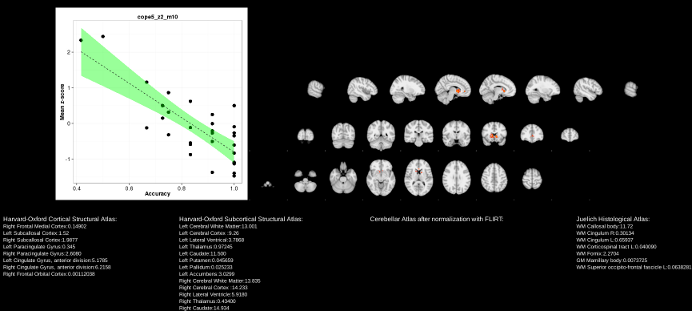
\includegraphics[scale=.6]{images/SSreport.png}
		\caption{Report plotting group FEAT results against behavioral measures.}
                \label{fig:fqresults}
	\end{center}
\end{figure}
\clearpage  \setcounter{codehighlight}{0}
